\documentclass[11pt,a4paper,twoside,openright]{report}

%  use packages
% --------------
\usepackage[utf8]{inputenc}
%~ \usepackage[T1]{fontenc}   % the font looks strange ...
\usepackage{geometry,amsmath, amsthm, amssymb}   % , units, dsfont, caption
% enumerate: \begin{enumerate}[{Example} I)] ... Roman numbering
\usepackage{graphicx,color,tabularx,float,subcaption,algorithmicx,algpseudocode,mathtools,textcomp}
\usepackage{multirow,emptypage,dcolumn,pdflscape}
\usepackage[super]{nth}
\usepackage[table]{xcolor}
\usepackage[titletoc]{appendix}
\usepackage{nomencl}
\makenomenclature

\usepackage[pdftex,
						pdftitle={Side-Channel Attack Analysis of AES White-Box Schemes, Jakub Klemsa},
						pdfauthor={Jakub Klemsa},
						pdfsubject={},
						pdfkeywords={White-Box AES, Side-Channel Attack},
						pdfcreator=pdflatex]{hyperref}

% fix left/right margins
\let\tmp\oddsidemargin
\let\oddsidemargin\evensidemargin
\let\evensidemargin\tmp
\reversemarginpar

\usepackage{fancyhdr}
	\pagestyle{fancy}
	\fancyhf{}
	\fancyhead[L]{\slshape \rightmark}   % \leftmark .. chapter
	\fancyhead[R]{\thepage}

%  customize
% -----------
\let\tmpitem\item
\renewcommand{\item}{\setlength{\itemsep}{0em}\tmpitem}   % míň roztahovačný seznamy
%~ \renewcommand{\labelitemi}{$\circ$}
%~ \newcommand*{\dittoclosing}{--- \raisebox{-0.5ex}{''} ---}   % use or not?

\let\epsilon\varepsilon
\let\phi\varphi

\setcounter{tocdepth}{1}
%~ \setcounter{secnumdepth}{4}

\renewcommand{\bibname}{References}
\renewcommand{\contentsname}{Table of Contents}
\renewcommand{\nomname}{Notations and Symbols}

%  theorems etc.
% ---------------
\theoremstyle{definition}
\newtheorem{thm}{Theorem}[chapter]
\newtheorem{lemma}[thm]{Lemma}
\newtheorem{thesis}[thm]{Thesis}
\newtheorem{conj}[thm]{Conjecture}
\newtheorem{cor}[thm]{Corollary}
\newtheorem{defn}[thm]{Definition}
\newtheorem{example}[thm]{Example}
\newtheorem{game}[thm]{Game}
\newtheorem{princ}[thm]{Principle}
\newtheorem{alg}{Algorithm}[chapter]

\theoremstyle{remark} 
\newtheorem{remark}[thm]{Remark}
\newtheorem{note}[thm]{Note}
\newtheorem{notion}[thm]{Notion}

%  my commands
% -------------
\renewcommand{\iff}{\Leftrightarrow}
\newcommand{\then}{\Rightarrow}
\newcommand{\rarr}{\rightarrow}
\newcommand{\larr}{\leftarrow}
\newcommand{\xor}{\oplus}
\newcommand{\unirand}{\xleftarrow{R}}
%~ \DeclareMathOperator*{\Prob}{\mathbb{Pr}}   % operátor* bude umět používat \limit :) ... \Pr už existuje! a \mathbb neumí malý písmena
\DeclareMathOperator*{\Adv}{Adv}
\DeclareMathOperator*{\AdvPRP}{Adv_{PRP}}
\DeclareMathOperator*{\AdvSS}{Adv_{SS}}
\DeclareMathOperator*{\AdvPRPSS}{Adv_{PRPSS}}
\DeclareMathOperator*{\bin}{bin}
\DeclareMathOperator*{\Corr}{Corr}
\DeclareMathOperator*{\Mean}{Mean}

\renewcommand{\P}{\mathbb{P}}
\newcommand{\GF}{\mathrm{GF}}
\newcommand{\N}{\mathbb{N}}
\newcommand{\Z}{\mathbb{Z}}
\newcommand{\R}{\mathbb{R}}
\newcommand{\C}{\mathbb{C}}
\newcommand{\Pclass}{\mathsf{P}}
\newcommand{\NPclass}{\mathsf{NP}}

\newcommand{\SubBytes}{\texttt{SubBytes}}
\newcommand{\ShiftRows}{\texttt{ShiftRows}}
\newcommand{\MixColumns}{\texttt{MixColumns}}
\newcommand{\AddRoundKey}{\texttt{AddRoundKey}}
\newcommand{\ExpandedKey}{\texttt{ExpandedKey}}
\newcommand{\KeySchedule}{\texttt{KeySchedule}}

\newcommand{\TBox}{\texttt{TBox}}
\newcommand{\MC}{\texttt{MC}}
\newcommand{\MB}{\texttt{MB}}
\newcommand{\IMB}{\texttt{IMB}}
\newcommand{\Enc}{\texttt{Enc}}

\newcommand{\nicefrac}[2]{{}^{#1}\!/_{#2}}
\newcommand{\atob}[2]{#1 , \ldots , #2}
\newcommand{\link}[1]{\href{http://#1}{\tt #1}}

\newcommand{\cg}[1]{\cellcolor{gray!#1}}

%%%%%%%%%%%%%%%%%%%%%%%%%%%%%%%%%%%%%%%%%%%%%%%%%%%%%%%%%%%%%%%%%%%%%%%%
%%%   k vyplnění ZAČÁTEK
%%%%%%%%%%%%%%%%%%%%%%%%%%%%%%%%%%%%%%%%%%%%%%%%%%%%%%%%%%%%%%%%%%%%%%%%

\newcommand{\cvut}{ČESKÉ VYSOKÉ UČENÍ TECHNICKÉ V~PRAZE}
\newcommand{\fjfi}{Fakulta jaderná a fyzikálně inženýrská}
\newcommand{\km}{Katedra matematiky}
\newcommand{\obor}{Matematická informatika}
\newcommand{\TYPPRACE}{DIPLOMOVÁ PRÁCE}
\newcommand{\TypPrace}{Diplomová práce}
\newcommand{\mePrace}{mé diplomové práce}
\newcommand{\kohoCoPraci}{ji}

\newcommand{\nazevcz}{Analýza AES white-box schémat pomocí útoku postranním kanálem}
\newcommand{\nazeven}{Side-Channel Attack Analysis of AES White-Box Schemes}
\newcommand{\autor}{Jakub Klemsa}
\newcommand{\vedouci}{prof. RNDr. Václav Matyáš, M.Sc., Ph.D.}
\newcommand{\vedoucimu}{prof. RNDr. Václavu Matyáši, M.Sc., Ph.D.}
\newcommand{\pracovisteVed}{Fakulta informatiky, Masarykova Univerzita}
\newcommand{\konzultant}{Mgr. Dušan Klinec}
\newcommand{\rok}{2016}
\newcommand{\akadRok}{2015/2016}
\newcommand{\misto}{Praha}
\newcommand{\VMiste}{V Praze}

\newcommand{\klicova}{Whitebox AES, útok postranním kanálem, paměťová stopa.}
\newcommand{\keyword}{White-Box AES, Side-Channel Attack, Memory Trace.}
\newcommand{\abstrCZ}{Samotný koncept whitebox kryptografie je relativně nový, přesto už známe některé silné teoretické výsledky. Z praktického pohledu se ale jednalo a jedná spíše o hru kočky s myší -- návrhy se neopírají o žádný známý těžký problém a tak bývá spíše otázkou času, jak dlouho vydrží vzdorovat snaze kryptanalytiků.

Velmi zajímavý a univerzální přístup \cite{bos2015differential} byl představen v preprintu na \link{iacr.org}. Cílem této práce je naprogramovat potřebné nástroje a útok reprodukovat, předně na implementaci z diplomové práce Dušana Klince \cite{klinec2013white}. Dále budeme zjišťovat, kudy informace uniká a jak tomu zabránit.}
\newcommand{\abstrEN}{Although the concept of White-Box Cryptography is quite recent, we already know some strong theoretical results. But from the practical point of view it rather reminds a cat-and-mouse game -- proposed schemes are not supported by any known computationally hard problem so it is usually a matter of time until it gets broken by cryptanalytic effort.

A very interesting and universal approach has been recently introduced in a paper \cite{bos2015differential} at \link{iacr.org}'s preprint. The goal of this thesis is to write required tools and reproduce the attack, especially on an implementation from Dušan Klinec's diploma thesis. Then we will identify where the point of leakage is and how to prevent from leaking the key.}

%%%%%%%%%%%%%%%%%%%%%%%%%%%%%%%%%%%%%%%%%%%%%%%%%%%%%%%%%%%%%%%%%%%%%%%%
%%%   k vyplnění KONEC
%%%%%%%%%%%%%%%%%%%%%%%%%%%%%%%%%%%%%%%%%%%%%%%%%%%%%%%%%%%%%%%%%%%%%%%%


\begin{document}


\pagenumbering{roman}
\begin{titlepage}
	
	%%% 1. úvodní strana
	\thispagestyle{empty}
	\begin{center}
		{\Large \cvut \\[12pt] \fjfi \\[260pt]}
		{\Huge \TYPPRACE}
	\end{center}
	\vfill
	{
		\Large \misto, \rok \hfill \autor
	}
	\cleardoublepage
	
	
	%%% 2. úvodní strana
	\thispagestyle{empty}
	\begin{center}
		{\Large \cvut \\[10pt] \fjfi \\[10pt] \km \\[40pt]}
		
\includegraphics[height=75pt]{lev.pdf} \\[100pt]
		
		{\LARGE \TYPPRACE \\[60pt]}
		
		{\Large\bf \nazevcz \\[30pt]}
		
		{\Large\bf \nazeven}
	\end{center}
	\vfill
	{
		\Large
		\begin{tabular}{ll}
		Vypracoval: & \autor\\[3pt]
		Školitel: & \vedouci\\[3pt]
		Akademický rok: & \akadRok
		\end{tabular}
	}
	\cleardoublepage
	
	
	%%% sem přijde ofic. zadání
	\thispagestyle{empty}
	\Large
	Na toto místo přijde svázat \textbf{zadání \mePrace}!
	
	\vspace{4mm}
	V~jednom z~výtisků musí být \textbf{originál} zadání, v~ostatních kopie.
	\normalsize
	\cleardoublepage
	
	
	%%% prohlášení
	\thispagestyle{empty}
	~
	\vfill
	\noindent\textbf{Čestné prohlášení}
	\vspace{0.5cm}
	
	\noindent
	Prohlašuji na tomto místě, že jsem předloženou práci vypracoval samostatně a že jsem uvedl veškerou použitou literaturu.
	\vspace{1.5cm}
	
	\noindent
	\vspace{5mm}\VMiste ~dne \today\hfill
		\begin{tabular}{c}
		. . . . . . . . . . . . . . . . . . . . . . .\\
		\autor
		\end{tabular}
	\cleardoublepage
	
	
	%%% poděkování
	\thispagestyle{empty}
	~
	\vfill
	\noindent\textbf{Poděkování}
	\vspace{0.5cm}
	
	\noindent
	Děkuji \vedoucimu, za vedení \mePrace ~a za podnětné návrhy, které \kohoCoPraci ~obohatily.
	
	\begin{flushright}
	\autor
	\end{flushright}
	\cleardoublepage
	
	
	%%% abstrakt atp.
	\thispagestyle{empty}
	\begin{tabularx}{\textwidth}{lX}
		{\em Název práce:} & \bf \nazevcz \\[4mm]
		{\em Autor:} & \autor \\[4mm]
		{\em Obor:} & \obor \\[4mm]
		{\em Druh práce:} & \TypPrace \\[4mm]
		{\em Vedoucí práce:} & \vedouci, \pracovisteVed \\[4mm]
		{\em Konzultant:} & \konzultant \\[4mm]
		{\em Abstrakt:} & \abstrCZ \\[4mm]
		{\em Klíčová slova:} & \klicova \\[20mm]
		
		{\em Title:} & \bf \nazeven \\[4mm]
		{\em Author:} & \autor \\[4mm]
		{\em Abstract:} & \abstrEN \\[4mm]
		{\em Keywords:} & \keyword
	\end{tabularx}
	\cleardoublepage
	
	
	%%% obsah
	\thispagestyle{empty}
	\tableofcontents
	\cleardoublepage
	
	
	%%% nomenklatura
	\thispagestyle{empty}
	\printnomenclature
	\cleardoublepage
	
\end{titlepage}

\pagenumbering{arabic}


%%%%%%%%%%%%%%%%%%%%%%%%%%%%%%%%%%%%%%%%%%%%%%%%%%%%%%%%%%%%%%%%%%%%%%%%
%%%   Z A Č Á T E K   P R Á C E
%%%%%%%%%%%%%%%%%%%%%%%%%%%%%%%%%%%%%%%%%%%%%%%%%%%%%%%%%%%%%%%%%%%%%%%%
		
		% FINAL CHECK:
		% 	abstrakty a keywords
		% 	V Praze dne \today -> český datum
		% 	\section{Capital Letters}
		% 	section \ref{...} -> Section \ref{...}
		% 	\mod vs \pmod
		% 	bib: title={{Bla Bla ... 2x závorky aby byly velký písmena}}
		% 	$SubBytes$ -> $\SubBytes$ ...
		% 	tables -> lookup tables
		% 	concatenation -- spelling
		% 	you vs. WE
		% 	an $8 ...
		% 	compose vs. concat !!!
		% 	E(k,m) instead of E(m,k)
		% 	adversary -> she
		% 	referred to as (-the?)
		% 	start -> begin with
		% 	závorky \left(\right)
		% 	setřídit nomenclaturu: \nomenclature[01]{$|S|$}{Cardinality of the set $S$}
		% 	| -> \mid (kde se hodí)
		% 	sofar -> so far
		% 	notion vs. notation
		% 	závorky \bigl( \bigr)
		% 	adversary vs. attacker
		% 	see vs. cf. (compare)
		% 	for this reason comma?
		% 	\Pr D E l k_a ??
		% 	e.g. -> e.g.\ 
		% 	všechno dát jako podmnožiny \{0,1\}^* !!!
		% 	přečíst si kydy z turku/sec eng a případně zařadit "historky z natáčení"
		% 	color box -> color-box
		% 	whitebox -> white-box
		% 	odkaz na section mimo chapter -> přidat chapter
		% 	introduced -> described (já asi těžko něco představil že ...)
		% 	hloubka obsahu?
		% 	opravdu dosmažit všechny 4 trace acq tooly
		% 	kam až číslovat? \subsubsection? změní \setcounter{secnumdepth}{4}
		% 	note vs. remark
		% 	XOR?
		% 	referencování na SCA algoritmy, neni lepší je pojmenovat?
		% 	polynomials in this thesis are with GF(2) coefficients, unless stated otherwise
		% 	projede vlna i Section~\ref{...} ??
		% 	
		
		
		%%% PŘEDMLUVA
		% cleardoublepage and phantomsection force that link jumps ABOVE heading, normally it would jump UNDER heading
\cleardoublepage\phantomsection

\addcontentsline{toc}{chapter}{Preface}
\chapter*{Preface}

Blah.

% PŘEDMLUVA !!! se tomu řiká u nás ...
%~ význam WBC, kde se to vzalo, co za útok že tam chci použít, musí to bejt poutavý!
% o čem ta práce vlastně bude ve smyslu uvedení do problému, jak/proč ta práce vznikla?

%~ Motivation for whitebox crypto, whitebox crypto history, milestones   % Bos et al. to hezky shrnul
	%~ from black-box ... gray-box ... white-box
	%~ malicious software on your device
	%~ cryptographic keys of third-parties
	%~ use cases: DRM
	%~ modeled as if adversary had full control over execution environment of the device running the implementation
	%~ everything allowed: perform static analysis, read/alter memory (fault injection)
	%~ Chow et al.\ \cite{chow2002aes}
	%~ program obfuscation impossibility results
	%~ goal of wbc = embed the secret key to the implementation s.t. it is difficult to extract it even when the source code is available
	%~ note the difference from obfuscation, in practice could be utilized as well
	%~ conjecture by Chow: wb implementations provide no long-term defense against attacks
	%~ symmetric crypto only, no published results on pubkey crypto
	%~ all published approaches have been broken
	%~ software vendors then disobey Kerckhoff's principle (cite) i.e. use secret design
	%~ Bos et al. exploit leaked information instead, no need for exact knowledge of design nor reverse engineering
	%~ perfect wb implementation should resist all existing and future side-channel attacks (C. Delerablee, T. Lepoint, P. Paillier, and M. Rivain. White-box security notions for symmetric encryption schemes. In T. Lange, K. Lauter, and P. Lisonek, editors, SAC 2013, volume 8282 of LNCS, pages 247–264, Burnaby, BC, Canada, Aug. 14–16, 2014. Springer, Berlin, Germany.)
	%~ ... Bos et al. utilize software traces for this purpose
	%~ The goal of this thesis is to reproduce the attack and make it easy for future researchers and analysis.

\section*{Work overview}
	
	\begin{description}
		\item[Chapter \ref{chap:intro}.] In this chapter we describe basic whitebox crypto techniques\ldots
		%~ \item[Chapter \ref{chap:results}.] This chapter presents our practical results together with\ldots
	\end{description}

% ====================================================================
% ====================================================================
% ====================================================================

A table for fun follows:
\begin{center}
\begin{tabular}{|| c || c | c | c ||}
	\hline\hline
	~ & \multicolumn{2}{c|}{\bf $n\times n$ squares} & {\bf Computational} \\
	~ & \multicolumn{1}{c}{Lower bound} & \multicolumn{1}{c|}{Upper bound} & {\bf Power}\\
	\hline
	2D & \multicolumn{2}{c|}{See see} & Universal \\
	\hline
	2D & see & see & Unknown \\
	\hline\hline
\end{tabular}
\end{center}

Just for fun:
\begin{figure}[H]
\begin{center}
	
\includegraphics[width=0.2\textwidth]{./figures/fig.pdf} % {šířka v mm}/370 je to původně
	\caption{Remove me, please.}
	\label{fig:3color}
\end{center}
\end{figure}

Or a multifigure:
\begin{figure}[H]
\begin{center}
	\begin{subfigure}[b]{0.2\textwidth}
		
\includegraphics[width=\textwidth]{./figures/fig.pdf}
		\caption{One.}
		\label{fig:one}
	\end{subfigure}
	\begin{subfigure}[b]{0.2\textwidth}
		
\includegraphics[width=\textwidth]{./figures/fig.pdf}
		\caption{Two.}
		\label{fig:two}
	\end{subfigure}
	\caption{One and Two.}
	\label{fig:onetwo}
\end{center}
\end{figure}

		
		%%% KAPITOLA 1
		\chapter{Introduction to White-Box Cryptography}
\label{chap:intro}

Before we introduce the concept of white-box cryptography, we present some introductory topics of cryptography itself -- we especially formalize notions of security. Then we describe the Advanced Encryption Standard \cite{fips2001aes} and an attempt for its white-box variant \cite{chow2002aes}.

\section{Introduction to Cryptography}
\label{sec:introcrypto}

%?% přesun mimo section přímo pod chapter?
% goal: introduce crypto in a broader context, yet not too much in detail
% starý jako lidstvo samo, bla bla, trochu ukázky z historie a jak to bylo špatný a jak se to umí lámat, security by obscurity, využívá cool matiku
% co po crypto vlastně chci
%~ crypto = basis for security mechanisms
%~ CONFIDENTIALITY and much more (e.g. integrity, digital signature, anonymity) or magic: zero knowledge proof of knowledge, FHE
%~  or a complicated construction of crypto primitives (e.g. digital currency, electronic election, electronic auction)
%~ 1. threat model (WB vs. BB later)
%~ 2. propose sth
%~ 3. prove that breaking it would break an underlying hard problem

\ldots\\
Let us imagine a typical situation where Alice wants to communicate with Bob confidentially over an insecure channel while Eve may eavesdrop on the channel. In the beginning, let us suppose that Alice and Bob share certain portion of secret information referred to as {\em secret key} and both control a secure execution environment where they intend to run their ciphering algorithm so that Eve can only observe what they send over the channel.

\begin{note}
\label{note:threat}
	The list of such attacker's abilities is referred to as {\em threat model}. Note that in the previous threat model the attacker is quite weak -- she can only read the traffic. If she were for instance able to manipulate the traffic, Alice and Bob would need to introduce another features to their protocol so that they could detect forged messages.
	
	Before we start introducing any means of security, we always need to identify the threat model first. For now we will only consider eavesdropping.
\end{note}

Our first intuitive requirements on Alice and Bob's ciphering algorithm could be expressed as follows: no matter what plaintext Alice and Bob encrypt and send over the channel, Eve shall {\em not} be able to
\begin{enumerate}
	\item recover any portion of any plaintext, \label{item:plainrecov}
	\item recover the secret key. \label{item:keyrecov}
\end{enumerate}
The item \ref{item:plainrecov} requirement is also referred to as {\em confidentiality}. Note that key recovery would lead to plaintext recovery as well, on the other hand not necessarily the other way around. Let us give an example of a primitive cipher.

\begin{example}
\label{ex:shift}
	{\em Shift cipher} is an ancient cipher used already by Julius Caesar and it works as follows: it inputs a string of letters from a finite alphabet $\cal A$, maps its letters bijectively to the numbers from $0$ to $|{\cal A}|-1$ and adds a constant $c\in\{\atob{0}{|{\cal A}|-1}\}$ modulo $|\cal A|$ to each number. Finally it maps the numbers back to letters yielding a string ``shifted'' by $c$ where $c$ can be interpreted as an element of $\cal A$ as well. Decryption can be done simply by substracting $c$ from the ciphertext in a similar way.
	
	Shift cipher can be easily broken by pen and paper only since there are as many keys as letters in the alphabet, typically $26$ english letters. You simply try them all until the plaintext makes sense. Such approach is referred to as {\em brute force attack} or {\em exhaustive search}.
\end{example}
\nomenclature{$\mid S\mid$}{Cardinality of the set $S$}

As we could see in the previous example, shift cipher is not much secure cipher. Therefore we would like to formalize the concept of cipher and its security.


% ==============================================================================
% ===   S Y M M E T R I C   A N D   A S Y M M E T R I C   C I P H E R        ===
% ==============================================================================

\subsection{Symmetric and Asymmetric Cipher}

There are two large families of ciphers -- symmetric and asymmetric. Shift cipher from Example \ref{ex:shift} belongs to the symmetric family which follows from the fact that it uses the same key for both encryption and decryption while asymmetric ciphers use distinct keys for encryption and decryption. Asymmetric ciphers are also referred to as public key ciphers but we will only consider symmetric ciphers in this thesis, a definition follows.

\begin{defn}[Symmetric Cipher]
\label{def:symcipher}
	Let $K$ denote the key space, $M$ the message space and $C$ the ciphertext space. {\em Symmetric cipher} is a pair of efficiently computable (possibly randomized) functions $(E,D)$, $E:K\times M\rarr C$, $D:K\times C\rarr M$, such that $\forall m\in M$ and $\forall k\in K$ it holds
	%~ \Pr\left(D(E(l,k),k)=l\right) = 1 . \label{eq:correct}
	\begin{equation}
		\Pr\Bigl(D\bigl(k,E(k,m)\bigr)=m\Bigr) = 1 . \label{eq:correct}
	\end{equation}
	%?% \footnote{In some use cases it might be useful to require only so called {\em overwhelming} probability; not needed in this thesis.}
\end{defn}
\nomenclature{$\Pr(\omega)$}{Probability of the event $\omega$}

\begin{note}
	Going back to Example \ref{ex:shift}, the key space is $\{\atob{0}{|{\cal A}|-1}\}\sim\cal A$, the message and ciphertext spaces are ${\cal A}^*$ which stands for the set of all strings over the alphabet $\cal A$.
\end{note}

According to the previous definition, we do not seem to have a definition of a proper cipher at all -- the only requirement is corectness (cf. Equation \ref{eq:correct}) -- but it totally lacks any security requirement. As we will see later, it is actually quite complicated to define ``security'' appropriately.


% ==============================================================================
% ===   I N F O R M A T I O N - T H E O R E T I C   A P P R O A C H          ===
% ==============================================================================

\subsection{Information-Theoretic Approach}

Shannon's groundbreaking work \cite{shannon1949mathematical} on the mathematics of communication gives us a tool -- information-theoretic approach. We can then define secure cipher as a cipher which outputs a ciphertext which carries no information about respective plaintext. Note that this can be rewritten in a more friendly form, a definition follows.

\begin{defn}[Perfectly Secure Cipher]
\label{def:perfsec}
	Let $(E,D)$ be a symmetric cipher. Then it is called {\em perfectly secure} if $\forall m_0,m_1\in M$ such that $|m_0| = |m_1|$ and $\forall c\in C$ it holds $\Pr\bigl(E(k,m_0)=c\bigr) = \Pr\bigl(E(k,m_1)=c\bigr)$ where $k$ is uniformly random in $K$, further denoted by $k\unirand K$.
\end{defn}
\nomenclature{$k\unirand K$}{$k$ is taken uniformly random from $K$}

\begin{note}
\label{note:indist}
	In other words, the attacker is not able to {\em distinguish} encryption of $m_0$ from encryption of $m_1$ by {\em any} means.
\end{note}

There is a cipher which is perfectly secure, see the following example.

\begin{example}[Vernam cipher]
	Let $K = M = C = \{0,1\}^n$ and $k\unirand K$. Given a plaintext $m$, {\em Vernam cipher} applies bitwise XOR of the key $k$ yielding ciphertext $c$ i.e. $c = m\xor k$.
\end{example}

\begin{note}
	Vernam cipher is also referred to as {\em One Time Pad} (OTP). Note that it is crucial that each key is only used once otherwise you can attack the cipher easily: given two ciphertexts using the same key $c_0=m_0\xor k$ and $c_1=m_1\xor k$, one can compute $c_0\xor c_1 = m_0\xor m_1$. This can be practically attacked using some apriori knowledge about plaintexts (e.g. encoding (ASCII), format and language of plaintext (XML and english) and so on) which reduces the amount of possibilities and typically leads to complete plaintext recovery.
\end{note}

Perfect security seems to be exactly what we want from a secure cipher but the following theorem shows that it implies certain inconveniences.

\begin{thm}
\label{thm:kgeqm}
	Let $(E,D)$ be a perfect cipher. Then $|K| \geq |M|$.
\end{thm}

\begin{note}
\label{note:intent}
	This consequence of perfect secrecy seems to go against our intention -- we would like to establish a shared secret key of a limited length and then, using the key, be able to encrypt as much information as we want. For this reason we need to weaken our security assumption. Note that previously there was no assumption on attacker's computing power -- the requirement was actually to hide the  plaintext from {\em any} attacker i.e. including an attacker with unlimited computing power.
\end{note}


% ==============================================================================
% ===   C O M P L E X I T Y - T H E O R E T I C   A P P R O A C H            ===
% ==============================================================================

\subsection{Complexity-Theoretic Approach}

We would like to utilize the fact that the attacker typically does not possess unlimited computing power but she can rather only solve probabilistic polynomial problems.

\begin{note}
\label{note:polyinterms}
	There arises a natural question: {\em Probabilistic polynomial in terms of what?} In cryptography, there is a meter for that referred to as {\em security parameter} which is typically the key-length. In the following text and for this purpose, the expression {\em effective} will be used frequently.
\end{note}

With this assumption, we can weaken our requirement on ciphertext from ``carries no information'' to ``is computationally impossible to gain some information''. In a manner analogous to Note \ref{note:indist}, we would like to make impossible to distinguish which plaintext has been encrypted, now considering an effective attacker only. We present this idea in the following game.

\begin{game}
\label{game:semsec}
	There are two parties -- a {\em challenger} and an {\em adversary}. First, the challenger chooses a random key $k\unirand K$ and a random bit $b\unirand\{0,1\}$. Then the adversary sends two equally long plaintexts $m_0$, $m_1$ of her choice to the challenger. The challenger then encrypts $m_b$ (according to $b$ she has chosen) and sends the resulting ciphertext $c$ back to the adversary. The adversary is allowed to perform multiple such queries while the challenger keeps constant key $k$ and bit $b$; the adversary is only limited by polynomial time.
	
	The aim of the adversary is to distinguish effectively which $b$ has been chosen by the challenger. See Figure \ref{fig:semsecgame} depicting this game.
\end{game}

\begin{note}
\label{note:semsec}
	Resistency of a cipher to this kind of attack is referred to as {\em semantic security}.
\end{note}

\begin{figure}[H]
\begin{center}
	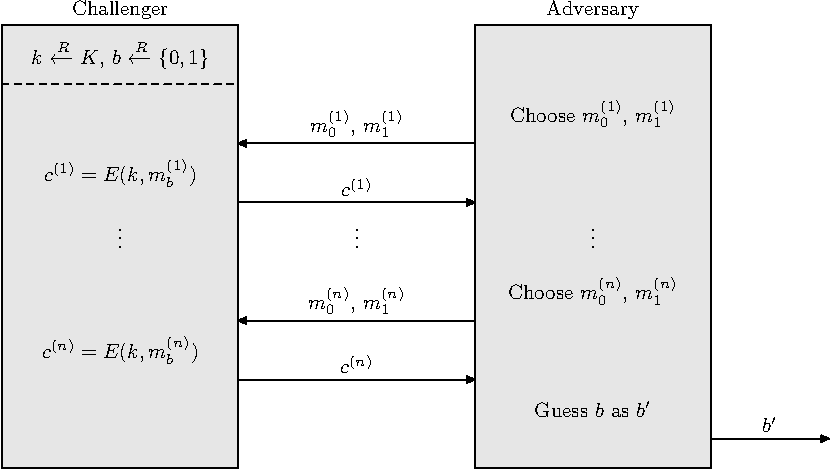
\includegraphics{./figures/game_semsec/game_semsec-1.pdf}
	\caption{Game \ref{game:semsec} depicted.}
	\label{fig:semsecgame}
\end{center}
\end{figure}

\subsubsection{Definition of Semantic Security}

Let us introduce some notion first.

\begin{defn}[Negligible Function]
\label{def:neglfunc}
	Let $\epsilon:\N\rarr\R$. $\epsilon$ is called {\em negligible} if $\forall d\in\N$ $\exists \lambda_0\in\N$ such that $\forall \lambda>\lambda_0$ it holds $\epsilon(\lambda)\leq\frac{1}{\lambda^d}$. In the opposite case, $\epsilon$ is called {\em non-negligible}.
\end{defn}
\nomenclature{$\N$}{Positive integers}
\nomenclature{$\R$}{Real numbers}

\begin{defn}[Overwhelming Function]
\label{def:overwh}
	Let $\epsilon:\N\rarr\R$. $\epsilon$ is called {\em overwhelming} if $1-\epsilon$ is negligible.
\end{defn}

\begin{note}
\label{note:neglconst}
	In practice, {\em negligible} is often used with concrete constants as well. $\epsilon<\frac{1}{2^{80}}$ is considered negligible i.e. events with such probability are not considered to occur during our lives, on the other hand $\epsilon>\frac{1}{2^{30}}$ is considered non-negligible i.e. it is likely to observe an event with such probability.
\end{note}

\begin{defn}[Oracle]
\label{def:oracle}
	Let $F:X\rarr Y$. {\em Oracle evaluating $F$} is a device which, given $x\in X$, evaluates and returns $F(x)$ in unit time, denoted by ${\cal O}_F$.
\end{defn}

\begin{defn}[Statistical Test]
\label{def:stattest}
	Let $F:X\rarr Y$. {\em Statistical test} is a (possibly randomized) effective algorithm $A$ which only has an access to an oracle evaluating $F$ and which outputs $0$ or $1$, denoted by $A({\cal O}_F)$.
\end{defn}

\begin{note}
	Statistical test will be also referred to as {\em adversary}.
\end{note}

\begin{defn}[Advantage]
\label{def:advant}
	Let $\cal F$, $\cal G$ be two distinct subsets of the set of all functions from $X$ to $Y$ and $A$ an adversary. We define {\em advantage} of adversary $A$ as
	\[
		\Adv(A,{\cal F},{\cal G}) = \left| \Pr\limits_{F\unirand {\cal F}}\bigl(A({\cal O}_F)=1\bigr) - \Pr\limits_{G\unirand {\cal G}}\bigl(A({\cal O}_G)=1\bigr) \right| .
	\]
\end{defn}

In other words, advantage tells us how likely adversary $A$ is able to distinguish a random function from one set of functions from a random function from another set based on its input/output behavior only. According to these sets, advantage can be ``customized'' for a specific purpose. Let us define such advantage for an adversary tempting to distinguish which of her plaintexts has been encrypted i.e. tells us how likely she is to win the Game \ref{game:semsec}.

\begin{defn}[Semantic Security Advantage]
\label{def:ssadvant}
	Let $E: K\times M\rarr C$ be an encryption function of a symmetric cipher, $k\unirand K$, ${\cal E}_b = \{E_b:M^2\rarr C \mid E_b(m_0,m_1) = E(k,m_b)\}$ for $b=0,1$ and $A$ an adversary. We define {\em semantic security advantage} of adversary $A$ as
	\[
		\AdvSS(A,E) = \Adv(A,{\cal E}_0,{\cal E}_1) .
	\]
\end{defn}

Semantic security advantage gives us a reasonable meter for formalization of Game \ref{game:semsec}. We use it to define another notion of security, cf.\ Definition \ref{def:perfsec} (Perfectly Secure Cipher).

\begin{defn}[Semantically Secure Cipher]
\label{def:semsec}
	Let $(E,D)$ be a symmetric cipher. Then it is called {\em semantically secure} if for {\em any} adversary $A$ the semantic security advantage $\AdvSS(A,E)$ is negligible.
\end{defn}

%!% přidat někam útok využívající zkrácení plaintextu po komprimaci
% it makes sense to compress -> encrypt but it might be insecure!

Semantically secure cipher therefore cannot be broken by any probabilistic-polynomial attack with overwhelming probability. On the other hand, it might be broken by an attacker with unlimited computing power unlike perfectly secure cipher which cannot be broken anyways, see Note \ref{note:indist}.

The benefit of semantic security over perfect security is that semantic security does not imply any inconvenient consequence analogous to Theorem \ref{thm:kgeqm} (i.e.\ addresses our intention as stated in Note \ref{note:intent}) and practically provides similar security.

Semantic security is usually achieved using smaller building blocks which are required to have certain properties. The following section describes a building block of one such possible approach.


% ==============================================================================
% ===   B L O C K   C I P H E R                                              ===
% ==============================================================================

\subsection{Block cipher}

There are two main approaches how to construct a semantically secure cipher. They make use of
\begin{enumerate}
	\item a {\em stream cipher}, or
	\item a {\em block cipher},
\end{enumerate}
respectively. Stream ciphers then achieve semantic security by proper initialization and block ciphers use initialization together with {\em modes of operation}, e.g.\ {\em Cipher Block Chaining} (CBC) or {\em Counter Mode} (CTR). Modes of operation will not be covered in this thesis; only block ciphers and their desired properties will be described, a bunch of definitions follows.

\begin{defn}[Pseudorandom Permutation]
\label{def:prp}
	Let $E: K\times X\rarr Y$. We call $E$ a {\em pseudorandom permutation} (PRP) if there exists an efficient algorithm which evaluates $E$, the function $E(k,\cdot): X\rarr Y$ is a bijection and there exists an efficient algorithm to compute $E^{-1}(k,\cdot)$ for every $k\in K$.
\end{defn}

\begin{note}
	%~ For $X$ and $Y$ being a set of fixed-length strings, e.g. $X = Y = \{0,1\}^n$   %?%
	Pseudorandom permutation is usually referred to as {\em block cipher}. Note that the previous definition is in some sense very similar to Definition \ref{def:symcipher} -- it does not introduce any security requirements either.
\end{note}

Pseudorandom permutations will play the main role from now and $k$ will play the role of their key. In order to achieve semantic security of certain constructions using a PRP, we need the PRP to behave like a truly random bijection. Let us demonstrate a possible approach on a game similar to Game \ref{game:semsec}.

\begin{game}
\label{game:prp}
	There are two parties -- a {\em challenger} and an {\em adversary}. Let $E:K\times X\rarr Y$ be a PRP. First, the challenger chooses a random key $k\unirand K$, a random bijection $F:X\rarr Y$ and a random bit $b\unirand\{0,1\}$. Then the adversary sends $x\in X$ of her choice to the challenger. The challenger then applies $E(k,\cdot)$ or $F$ if $b=0$ or $1$, respectively, and sends the result back to the adversary. The adversary is allowed to perform multiple such queries again.
	
	The aim of the adversary is to distinguish effectively which $b$ has been chosen by the challenger.
\end{game}

Before we give a formal definition of a secure PRP, we define adversary's advantage in the previous game in a manner analogous to Definition \ref{def:ssadvant}.

\begin{defn}[PRP Advantage]
\label{def:prpadvant}
	Let $E: K\times X\rarr Y$ be a PRP, $\cal B$ the set of all bijections from $X$ to $Y$ and $A$ an adversary. We define {\em PRP advantage} of adversary $A$ as
	\[
		\AdvPRP(A,E) = \Adv\Bigl(A,\bigl\{E(k,\cdot)\bigm|k\in K\bigr\},{\cal P}\Bigr) .
	\]
\end{defn}

PRP advantage tells us how likely adversary $A$ is able to distinguish a PRP with a random key from a truly random bijection based on its input/output behavior only. The definition of secure PRP follows.

\begin{defn}[Secure PRP]
\label{def:secprp}
	Let $E: K\times X\rarr Y$ be a PRP. Then $E$ is called {\em secure PRP} if for {\em any} adversary $A$ the PRP advantage $\AdvPRP(A,E)$ is negligible.
\end{defn}

In other words, given a random key, PRP is secure if it is computationaly indistinguishable from a truly random bijection. 

%!% diffusion vs. confusion
% prej Shannon: Communication Theory of Secrecy Systems

An example covering most introduced concepts follows.

\begin{example}
	Let $E:\{0,1\}^{128}\times\{0,1\}^{128}\rarr\{0,1\}^{128}$ be a PRP defined as
	\[
		E(k,x) = \bin\bigl((k)_2 + (x)_2 \mod{2^{128}}\bigr)
	\]
	where $\bin(\cdot)$ stands for number's $128$-bit binary representation and $(\cdot)_2$ stands for a number represented by given binary string.
	
	Now let us construct an adversary $A$ as follows: it generates two arbitrary but distinct $x_0,x_1\in\{0,1\}^{128}$ and feeds them to an oracle computing either PRP $E$ or a truly random bijection. The oracle returns $y_0$ and $y_1$, respectively, and the adversary compares values $(y_i)_2 - (x_i)_2 \mod{2^{128}}$ for $i=0,1$ with each other. If these values are equal, $A$ returns $1$, $0$ otherwise.
	
	Note that if the oracle computes PRP $E$ then these values are always equal. Otherwise, i.e. the oracle computes a truly random bijection, the values are distinct with overwhelming probability. Therefore the PRP advantage of such adversary is
	\[
		\AdvPRP(A,E) = \left| \Pr\limits_{k\unirand \{0,1\}^{128}}\Bigl(A\bigl({\cal O}_{E(k,\cdot)}\bigr)=1\Bigr) - \Pr\limits_{P\unirand {\cal B}}\Bigl(A({\cal O}_P)=1\Bigr) \right| = 1 - \epsilon
	\]
	where $\cal B$ stands for the set of all bijections on $\{0,1\}^{128}$ and $\epsilon$ is negligible.
	
	It follows that such PRP is totally insecure since there exists an attacker with overwhelming advantage but only a negligible advantage is allowed so that PRP is secure.
\end{example}

\begin{note}
\label{note:secbyobsc}
	In the previous example, the adversary exploits the knowledge of the cipher's internal structure -- she knows everything but the key. One could have an idea to hide the structure from the attacker but this is actually a {\em very} bad idea. Once your construction leaks, you need to deploy a new ciphering algorithm confidentially but you have no way how to do so.
	
	You shall rather use a secure publicly known cipher and only rely on the key. Once your key is compromised, you simply establish a new key. Also note that your key is only to be protected within your device but the ciphering algorithm would have to be protected globally.
	
	Such approach hiding the design of a cipher is referred to as {\em security by obscurity} and shall be strictly avoided.
\end{note}

This idea has already been addressed in 1883 by Kerckhoffs \cite{auguste1883cryptographie}. It is usually referred to as {\em Kerckhoffs's Principle} and its six rules follow (originally french, english translation taken from \cite{petitcolas2016kerckhoffs}):
\begin{princ}[Kerckhoffs]
	~
	\begin{enumerate}
		\item The system must be substantially, if not mathematically, undecipherable;
		\item The system must not require secrecy and can be stolen by the enemy without causing trouble;\label{item:kerck}
		\item It must be easy to communicate and retain the key without the aid of written notes, it must also be easy to change or modify the key at the discretion of the correspondents;
		\item The system ought to be compatible with telegraph communication;
		\item The system must be portable, and its use must not require more than one person;
		\item Finally, given the circumstances in which such system is applied, it must be easy to use and must neither stress the mind or require the knowledge of a long series of rules.
	\end{enumerate}
\end{princ}
Hence harming rule \ref{item:kerck} from the previous list leads to security by obscurity as introduced in Note \ref{note:secbyobsc}.


% ==============================================================================
% ===   P R O V A B L E   S E C U R I T Y   P R O O F S                      ===
% ==============================================================================

\subsection{Provable Security Proofs}

Now we know what it is a secure PRP (or a secure block cipher) -- it is based on Game \ref{game:prp} where the aim of the adversary is to distinguish a PRP from a truly random bijection. The obvious question is what happens if we put a secure PRP into Game \ref{game:semsec} where the adversary tries distinguish which of his two inputs has been processed by a cipher. Note that PRP is a cipher (cf. Definition \ref{def:symcipher} and \ref{def:prp}) so it makes a sense. Indeed, given a PRP, there exists an effective algorithm evaluating it and since it is invertible, also Equation \ref{eq:correct} holds.

\begin{note}
\label{note:singleaccess}
	A drawback of PRPs is that they cannot be randomized, therefore we will need to limit the amount of adversary-challenger queries to one or, equivalently, change the key after each query. If we do not do so then there exists a trivially winning adversary $A$.
	
	Indeed, such adversary picks three distinct plaintexts $m_0$, $m_1$, $m_2$ (well, let us suppose there are at least three plaintexts in $M$) and sends $(m_0,m_1)$ to the challenger while she gets back some ciphertext $c_a$. In her second query, the adversary sends $(m_0,m_2)$ to the challenger and receives another ciphertext, let say $c_b$. Since PRP is a deterministic bijection, she can decide with certainty:
	\begin{itemize}
		\item $b=0$ if $c_a = c_b$, or
		\item $b=1$ if $c_a \neq c_b$
	\end{itemize}
	and win the game with $\AdvSS(A,E) = 1$ where $E$ stands for the PRP.
\end{note}

\begin{note}
\label{note:randomize}
	The previous note also implies that in order to achieve semantic security of a cipher, the cipher {\em must} encrypt the same plaintext differently each time. This can be achieved using randomization or counters, both approaches are practically used.
\end{note}

Let us modify Game \ref{game:semsec} in a manner described within Note \ref{note:singleaccess} for the purpose of testing PRPs.

\begin{game}
\label{game:semsecprp}
	There are two parties -- a {\em challenger} and an {\em adversary}. Let $E:K\times X\rarr Y$ be a PRP. First, the challenger chooses a random bit $b\unirand\{0,1\}$ and before each round also a random key $k\unirand K$. In each round the adversary sends two equally long plaintexts $m_0$, $m_1$ of her choice to the challenger. The challenger then computes $c = E(k,m_b)$ and sends it back to the adversary. Note that the adversary is allowed to perform multiple queries again but, unlike the previous games, the key changes over and over again.
	
	The aim of the adversary is to distinguish effectively which $b$ has been chosen by the challenger.
\end{game}

\begin{note}
\label{note:semsecprp}
	Based on the previous game, we could define {\em PRP semantic security advantage} ($\AdvPRPSS$) and {\em semantically secure PRP} (cf. Game \ref{game:semsec}, Definitions \ref{def:ssadvant} and \ref{def:semsec}). The difference would be that the oracle access should be redefined -- it would either need to be limited to one or the oracle would need to change the function it evaluates. Due to these technical obstacles we do not provide exact definitions.
\end{note}

The following theorem gives a connection between Game \ref{game:prp} and \ref{game:semsecprp}. It claims that given a PRP $E$ winning Game \ref{game:prp} i.e. $E$ is indistinguishable from a truly random bijection, $E$ wins Game \ref{game:semsecprp} as well i.e. no adversary can distinguish encryption of $m_0$ from encryption of $m_1$.

\begin{thm}
\label{thm:semsecprp}
	Let $E: K\times X\rarr Y$ be a secure PRP. Then it is also a semantically secure PRP.
\end{thm}
\begin{proof}
	We show that for every PRP semantic security adversary $A$ there exist PRP security adversaries $B_0$, $B_1$ such that
	\begin{equation}\label{eq:aleqbb}
		\AdvPRPSS(A,E) \leq \AdvPRP(B_0,E) + \AdvPRP(B_1,E) .
	\end{equation}
	The claim then follows -- if $E$ is a secure PRP i.e. $\AdvPRP(B_0,E) + \AdvPRP(B_1,E)$ is negligible then also $\AdvPRPSS(A,E)$ is negligible, therefore $E$ is a semantically secure PRP.
	
	Let us first denote $W_b$ the event when adversary $A$ answers $1$ while the true value of the PRP semantic security game is $b$ for $b=0,1$. In this notation it holds
	\begin{equation}\label{eq:prpssae}
		\AdvPRPSS(A,E) = \bigl| \Pr(W_1) - \Pr(W_0) \bigr| .
	\end{equation}
	Let us further denote $R_b$ the same event with only difference -- the PRP semantic security game uses a random bijection instead. It holds
	\begin{equation}\label{eq:rr0}
		\bigl| \Pr(R_1) - \Pr(R_0) \bigr| = 0
	\end{equation}
	since $b\unirand\{0,1\}$ and both $R_b$ provide a truly random bijection independent from $b$.
	
	Now we construct adversaries $B_0$, $B_1$ distinguishing PRPs from truly random ones while we make use of adversary $A$. Let us construct $B_0$ first. We ask $A$ to provide $m_0$ and $m_1$, then we feed the oracle with $m_0$ obtaining $c$ as a result. Note that either $c=E(k,m_0)$ or $c=F(m_0)$ according to $b$ where $F$ is a truly random bijection. We provide this $c$ to adversary $A$ and output what $A$ outputs. The advantage of adversary $B_0$ is
	\begin{equation}\label{eq:prpb0}
		\AdvPRP(B_0,E) = \left| \Pr(W_0) - \Pr(R_0) \right| .
	\end{equation}
	We construct $B_1$ in a similar manner (i.e.\ choosing $m_1$ instead) and get
	\begin{equation}\label{eq:prpb1}
		\AdvPRP(B_1,E) = \left| \Pr(W_1) - \Pr(R_1) \right| .
	\end{equation}
	Combining Equations \ref{eq:prpssae}, \ref{eq:rr0}, \ref{eq:prpb0} and \ref{eq:prpb1} we get
	\begin{align*}
		\AdvPRPSS(A,E) &= \left| \Pr(W_1) - \Pr(W_0) \right| \leq \\
		&\leq \left| \Pr(W_1) - \Pr(R_1) \right| + \left| \Pr(W_0) - \Pr(R_0) \right| = \\
		&= \AdvPRP(B_1,E) + \AdvPRP(B_0,E)
	\end{align*}
	which finally proves Equation \ref{eq:aleqbb}.
\end{proof}

\begin{note}
	A semantically secure PRP does not need to be a secure PRP. Indeed, let $E: K\times X\rarr Y$ be a secure PRP and define $E'(k,x) = E(k,x)\|1$ where $\|$ stands for string concatenation. $E'$ is obviously semantically secure (it remains hard to distinguish encryptions of dinstinct plaintexts) but it can be easily distinguished from a truly random bijection since it always ends with $1$. Advantage of such adversary would be $\AdvPRP(A,E') = \nicefrac{1}{2}$ which is clearly non-negligible.
\end{note}

The previous theorem is especially important for the idea behind its proof which is used in many other proofs related to provable-security. In this proof we construct adversaries $B_0$, $B_1$ which internally employ adversary $A$ and then we use advantage of $A$ to estimate advantages of $B_0$ and $B_1$.


% ==============================================================================
% ===   P R O V A B L E   V S   R E A L - W O R L D                          ===
% ==============================================================================

\subsection{Provable vs. Real-World Security}
\label{sec:provable}

Provable security is one aspect, the other is practical construction of a cipher. Note that there is no provably secure block cipher known.

If there were, it would actually imply that $\Pclass \subsetneq \NPclass$ which is an open millenium problem. Indeed, if $\Pclass = \NPclass$ and $E$ were a PRP, then the adversary could, given certain (polynomial) amount of plaintext-ciphertext pairs $(m_i,c_i)$, look for a key $k$ such that $c_i = E(k,m_i)$ for all $i$. Then she would simply answer ``truly random'' if no such $k$ was found, otherwise she says ``pseudorandom''. Here the ``truly random'' answer is sure while the ``pseudorandom'' answer is just a conjecture but with sufficiently large probability.
\nomenclature{$\Pclass$}{Deterministic polynomial complexity class i.e. the set of decision problems which can be solved by a deterministic Turing machine in polynomial time}
\nomenclature{$\NPclass$}{Non-deterministic polynomial complexity class i.e. the set of decision problems which can be solved by a non-deterministic Turing machine in polynomial time}

Instead, real-world block ciphers are {\em beleived} to be secure based on a simple fact: no known attack is far better than exhaustive search. One such block cipher is called {\em Advanced Encryption Standard} (AES) and will be of top interest in this thesis. AES will be described in detail in Section \ref{sec:aes}.


% ==============================================================================
% ===   F R O M   B L A C K - B O X   T O   W H I T E - B O X                ===
% ==============================================================================

\subsection{From Black-Box to White-Box Attack Context}
\label{sec:bbtowb}

The other central topic of this thesis is {\em white-box attack context}. In order to explain what it is, let us start with {\em black-box attack context}.

\subsubsection{Black-Box}

First of all, as stated in Note \ref{note:threat}, we need to address attacker's abilities -- the threat model. In the black box model, the attacker is given an access to an oracle (see Definition \ref{def:oracle}) evaluating given encryption algorithm $E$ with a random secret key $k$ while the (primary) goal of the attacker is to recover the key. The attacker has absolutely no information but inputs and respective outputs, she cannot observe any internal routines of encryption, hence black box.

\begin{note}
	There could be many other goals than just key recovery, e.g. guessing the ciphertext in advance or be able to decrypt certain/given ciphertext with non-negligible probability and so on. Actually whatever you can imagine which could be in principle possible with a PRP but could not be possible with a truly random bijection.
\end{note}

Classical ciphers are designed under the assumption of black-box attack context thus their implementation must be extremely careful. The attacker could for example measure the time of encryption and exploit this information which was not considered during the design of the cipher.

\subsubsection{Gray-Box}

Gray-box attack context is closer to the reality since we do not encrypt using oracles but rather using some physical devices which run a specific implementation of given cipher. In the gray box model, cipher is thus supposed to be implemented and run while the attacker can observe some information related to cipher's byproducts as well.

Such information leaks can be modelled as a set of distributions conditioned by byproducts and are referred to as {\em leakage model}. There is an area of theoretical cryptography studying leakages -- {\em Leakage Resilient Cryptography}. A practical attack exploiting such leaks will be described in Chapter \ref{chap:attack} in Section \ref{sec:side}.   %?% LRC introduced by?

\subsubsection{White-Box}

Finally there is the most extreme case where the attacker has full control over the execution environment -- the white-box attack context. Full control means that the attacker can step the algorithm and directly observe and alter byproducts in the memory or even skip, alter and insert instructions. Clearly, the key cannot be kept in its original form, it must be somehow hidden but still usable for encryption.


% previously: Finally there is the most extreme case where the attacker has full control over the execution environment -- the white-box attack context. Full control means that the attacker can step the algorithm and directly observe and alter byproducts in the memory or even skip, alter and insert instructions. Clearly, the key cannot be kept in its original form, it must be somehow hidden but still usable for encryption.

\section{White-Box Cryptography}
	
	
	
%~ detailně popsat kde se vzala vč. citací, vývoj, hra na kočku a myš, impos. results
%~ že neni žádnej public key wb

% je to de facto threat model
%~ straightforward AES implementation is totally insecure if certain byproducts or even some information related to them is revealed. An attack exploiting such information leaks is covered in detail in Section \ref{sec:side}.

% implementation can help, e.g. timing attacks
% RSA, an asymmetric cipher, could serve as a good example
% black box: like an oracle, everything holds. ciphers designed wrt black box, why wb? what it is? ...

%~ diffusion vs. confusion


\section{Advanced Encryption Standard}
\label{sec:aes}

In 1997, Curtin and Dolske were the first to publicly announce \cite{curtin1998brute} that they have cracked Data Encryption Standard (DES, \cite{fips1977des}) -- a symmetric block cipher which had been in use for $20$ years. In the same year, the National Institute of Standards and Technology (NIST) initiated a selection process for a new encryption standard. During the process, DES was partially replaced with Triple-DES described in ANSI draft X9.52 \cite{americantripple}.

In 1998, NIST chose $15$ candidates and asked cryptology community for help with analyzing the candidates. After a careful analysis, NIST proposed Rijndael\footnote{From authors' names: Vincent Rijmen and Joan Daemen.} \cite{daemen1999aes} as the new standard called {\em Advanced Encryption Standard} (AES) \cite{fips2001aes} on November 26, 2001. The standard specifies the Rijndael algorithm with block-length of $128$ bits and key-lengths of $128$, $192$ and $256$ bits. Note that the original Rijndael algorithm \cite{daemen2013rijndael} describes more block- and key-length variants. On the other hand, we will only consider its $128$-$128$-bit variant in the following text, unless stated otherwise.

Today, alomst 15 years later, AES is used worldwide and, although extensively analysed, it is still beleived to have considerable security margin.


% ==============================================================================
% ===   A E S   A L G O R I T H M   P R E R E Q U I S I T I E S              ===
% ==============================================================================

\subsection{AES Algorithm Prerequisities}

AES encryption\footnote{Decryption will be treated separately at the end of this section.} consists of $10$ rounds, each round (except for the last one) consists of $4$ different operations which will be described later. All of these operations work with $128$-bit words, let us call them {\em states}. Before we start, let us consider a few different state representations. 

First we split its $128$ bits into $16$ bytes denoted by $A_{0,0}$, $A_{1,0}$, $A_{2,0}$, $A_{3,0}$, $A_{0,1}$, $\ldots$, $A_{3,1}$, $\ldots$, $A_{3,3}$, respectively, obtaining a $4\times 4$ array where $A_{i,j}$ stands for an element in $i$-th row and $j$-th column.

\begin{remark}
\label{rem:aesstate}
	Note that the order of bytes in the state fills the array in a column-first manner assuming standard row/column order of indexes.
\end{remark}

Let us further denote $F = \GF(2)[x]/x^8+x^4+x^3+x+1$ which is a field of polynomials with integral coefficients reduced$\mod 2$ i.e. $0$, $1$, these polynomials are further reduced$\mod(x^8+x^4+x^3+x+1)$. This field has $2^8$ elements and is usually referred to as {\em Rijndael's field}. In AES context it might be denoted also by $\GF(2^8)$.

\nomenclature{$\GF(p^n)$}{Galois Field with $p^n$ elements, $p$ prime}
\nomenclature{$F[x]$}{Ring of polynomials over $F$}

Each byte $A_{i,j} = a_7a_6\ldots a_0$, $a_i\in\GF(2)$, is then considered as an element of $F$ simply as $a_7x^7 + a_6x^6 + a_5x^5 + a_4x^4 + a_3x^3 + a_2x^2 + a_1x + a_0$.  Note that byte may also be written in hexadecimal notation and still considered as an element of $F$. See Figure \ref{fig:aesnot} with a few of possible AES state representations.

\begin{figure}[H]
\[
\arraycolsep=.5em\def\arraystretch{1.5}
	01010001\,11010110\,\ldots\;\sim\;\texttt{51}\,\texttt{d6}\,\ldots\;\sim\;
	\begin{array}{|c|c|c|c|}
		\hline
		x^6 + x^4 + 1 & \ldots & \ldots & \ldots \\
		\hline
		x^7 + x^6 + x^4 + x^2 + x & \ldots & \ldots & \ldots \\
		\hline
		\ldots & \ldots & \ldots & \ldots \\
		\hline
		\ldots & \ldots & \ldots & \ldots \\
		\hline
	\end{array}
\]
\caption{A few of possible AES state representations.}
\label{fig:aesnot}
\end{figure}

\noindent
Now let us move on to definitions of the $4$ operations.

\subsubsection{SubBytes}
	
	$\SubBytes$ operation is often referred to as {\em SBox} and denoted by $S$. It is defined byte-wise, i.e. $S: F \rightarrow F$. For $A\in F$, let $A'$ stand for
	\begin{itemize}
		\item $A^{-1}$, if $A \neq 0$,
		\item $0$, if $A = 0$.
	\end{itemize}
	
	\begin{note}
	\label{note:rijinv}
		Even though $A'$ is not a proper field inverse, it is often referred to as inverse in Rijndael field or Rijndael inverse of $A$. Note that it is invertible.
	\end{note}
	
	Before we define $\SubBytes$ we have to emphasize that the following multiplication is {\em not} performed in $F$ but in the ring of binary polynomials $\GF(2)[x]$ instead. $\SubBytes$ is defined as follows:
	\newcommand{\defsbox}{S(A) = (x^4 + x^3 + x^2 + x + 1) \cdot A' + x^6 + x^5 + x + 1 \pmod{x^8+1}}
	\begin{equation}
	\label{eq:sbox}
		\defsbox .
	\end{equation}
	
	\begin{note}
	\label{note:sboxinv}
		Although $x^8+1$ is not irreducible (it holds $x^8+1 = (x+1)^8$), $x^4 + x^3 + x^2 + x + 1$ is coprime with $x^8+1$, therefore it has an inverse$\mod(x^8+1)$. It follows that $\SubBytes$ is an invertible bijection.
	\end{note}
	
	$\SubBytes$ is the only source of nonlinearity in AES thus it shall have excellent nonlinearity properties. This was the major weakness of DES, its predecessor. A practical linear attack against DES was introduced by Matsui in 1993 \cite{matsui1994linear} and analyzed in detail and successfuly performed by Junod in 2001 \cite{junod2001complexity}.
	
	\begin{note}
	\label{note:sboxtable}
		Since $\SubBytes$ has only $256$ possible inputs, it is usually precomputed and implemented as a lookup table, obviously for performance reasons.
	\end{note}
	
	The reason why $\SubBytes$ was not introduced the other way around (i.e.\ as a lookup table with good non-linearity properties) is the simple algebraic form of $S$ which enables mathematical analysis as well as statistical.   %?% dát do appendixu tabulku?

\subsubsection{ShiftRows}
	
	$\ShiftRows$ operation is very simple -- it only cyclically shifts rows of the state array. It moves $i$-th row by $i$ positions to the left where rows are numbered from $0$; see Figure \ref{fig:shiftrows}. Note that row entries are not next to each other in AES state, see Remark \ref{rem:aesstate}. $\ShiftRows$ is obviously invertible.
	
	\begin{figure}[H]
	\[
	\arraycolsep=.5em\def\arraystretch{1.5}
		\begin{array}{|c|c|c|c|}
			\hline
			A_{0,0} & \cg{.92} A_{0,1} & \cg{.84} A_{0,2} & \cg{.76} A_{0,3} \\
			\hline
			A_{1,0} & \cg{.92} A_{1,1} & \cg{.84} A_{1,2} & \cg{.76} A_{1,3} \\
			\hline
			A_{2,0} & \cg{.92} A_{2,1} & \cg{.84} A_{2,2} & \cg{.76} A_{2,3} \\
			\hline
			A_{3,0} & \cg{.92} A_{3,1} & \cg{.84} A_{3,2} & \cg{.76} A_{3,3} \\
			\hline
		\end{array}
		\quad\xrightarrow{\ShiftRows}\quad
		\begin{array}{|c|c|c|c|}
			\hline
			A_{0,0} & \cg{.92} A_{0,1} & \cg{.84} A_{0,2} & \cg{.76} A_{0,3} \\
			\hline
			\cg{.92} A_{1,1} & \cg{.84} A_{1,2} & \cg{.76} A_{1,3} & A_{1,0} \\
			\hline
			\cg{.84} A_{2,2} & \cg{.76} A_{2,3} & A_{2,0} & \cg{.92} A_{2,1} \\
			\hline
			\cg{.76} A_{3,3} & A_{3,0} & \cg{.92} A_{3,1} & \cg{.84} A_{3,2} \\
			\hline
		\end{array}
	\]
	\caption{$\ShiftRows$ operation on a state array.}
	\label{fig:shiftrows}
	\end{figure}
	
	The design motivation is to introduce inter-column diffusion. Note that $\ShiftRows$ does not diffuse bytes internally -- the following operation is here for this purpose.

\subsubsection{MixColumns}
	
	$\MixColumns$ operates on the state array in a column-wise manner. Let us pick a column from the state array and denote its elements by $A_0, A_1, A_2, A_3$, respectively. $\MixColumns$ considers it as a polynomial $a(z) = A_0 + A_1 z + A_2 z^2 + A_3 z^3$ -- an element of $F[z]$. Let $b(z)$ denote the output of $\MixColumns$, then it is defined as
	\begin{equation}
	\label{eq:mixcolpoly}
		b(z) = c(z) \cdot a(z) \pmod{z^4+1}
	\end{equation}
	where $c(z) = \texttt{03}\cdot z^3 + \texttt{01}\cdot z^2 + \texttt{01}\cdot z^2 + \texttt{02}$. Note that here we used hexadecimal notation for elements of $F$ which could also be viewed as polynomials. To avoid confusion, we used $z$ instead of $x$.
	
	Note that $c(z)$ is coprime with $z^4+1$ therefore invertible$\mod{z^4+1}$, it follows that $\MixColumns$ is invertible. 
	The goal of $\MixColumns$ is to introduce inter-byte diffusion within a column.
	
	Later we will make use of its different, linear algebra representation. Let us denote $b(z) = B_0 + B_1 z + B_2 z^2 + B_3 z^3$. Modular multiplication in Equation \ref{eq:mixcolpoly}, which is performed in $F[z]$, can be rewritten into matrix multiplication back in $F$, indeed
	\begin{equation}
	\label{eq:mixcolmatr}
		\begin{pmatrix}
			B_0 \\ B_1 \\ B_2 \\ B_3
		\end{pmatrix}
		=
		\begin{pmatrix}
			\texttt{02} & \texttt{03} & \texttt{01} & \texttt{01} \\
			\texttt{01} & \texttt{02} & \texttt{03} & \texttt{01} \\
			\texttt{01} & \texttt{01} & \texttt{02} & \texttt{03} \\
			\texttt{03} & \texttt{01} & \texttt{01} & \texttt{02}
		\end{pmatrix}
		\begin{pmatrix}
			A_0 \\ A_1 \\ A_2 \\ A_3
		\end{pmatrix}.
	\end{equation}

\subsubsection{AddRoundKey}
	
	Given a $128$-bit round key, $\AddRoundKey$ operation simply bitwise XORs it on the state. The round key is derived from the encryption key using $\KeySchedule$ routine which follows.
	
	$\AddRoundKey$ is the only step which employs keying material. Note that it is its own inverse.

\subsubsection{KeySchedule}
	
	$\KeySchedule$ is a routine which expands $128$-bit encryption key into $11$-times longer $\ExpandedKey$. $128$-bit blocks of $\ExpandedKey$ will serve as round keys. Their position within $\ExpandedKey$ will be indexed from $0$.
	
	\begin{note}
	\label{note:expkey}
		The most important consequence for us is that $\ExpandedKey$ begins with plain encryption key.
	\end{note}
	
	We omit further details here because $\KeySchedule$ is specified rather in algorithmic than algebraic manner, see \cite[pp.43-45]{daemen2013rijndael} for detail.


% ==============================================================================
% ===   A E S   A L G O R I T H M   D E S C R I P T I O N                    ===
% ==============================================================================

\subsection{AES Algorithm Description}

AES, as already stated, consists of $10$ rounds of $4$ operations except for the last one where $\MixColumns$ is missing, see the following algorithm.

\begin{alg}
\label{alg:aes}
	Given a $128$-bit plaintext and a key, return its AES encryption.
	\begin{algorithmic}[1]
		\Function{AES\_Encryption}{$Plaintext,Key$}
			\State $\ExpandedKey \gets \KeySchedule(Key)$
			\State $State \gets Plaintext$ \label{line:stateplain}
			\State $\AddRoundKey(State, \ExpandedKey[0])$ \label{line:addrk}
			\For{$Round = 1 \to 9$}
				\State $\SubBytes(State)$
				\State $\ShiftRows(State)$
				\State $\MixColumns(State)$
				\State $\AddRoundKey(State, \ExpandedKey[Round])$
			\EndFor
			\State $\SubBytes(State)$
			\State $\ShiftRows(State)$
			\State $\AddRoundKey(State, \ExpandedKey[10])$
			\State\Return $State$
		\EndFunction
	\end{algorithmic}
\end{alg}

\begin{note}
	Since we have commented on every step about how it can be inverted, AES encryption algorithm is hence also invertible. We get AES decryption algorithm by executing inverse counterparts of AES encryption steps in reverse order.
\end{note}


% ==============================================================================
% ===   A E S   I M P L E M E N T A T I O N   N O T E                        ===
% ==============================================================================

\subsection{AES Implementation Note}
\label{sec:aeslookup}

As stated in Note \ref{note:sboxtable}, $\ShiftRows$ can be implemented as a lookup table for performance reasons. Unlike $\SubBytes$, $\MixColumns$ operates on a substantially larger domain, therefore cannot be directly implemented as a lookup table. But we can utilize its matrix representation, see Equation \ref{eq:mixcolmatr}. Let us denote
\[
	\C =
	\begin{pmatrix}
		\texttt{02} & \texttt{03} & \texttt{01} & \texttt{01} \\
		\texttt{01} & \texttt{02} & \texttt{03} & \texttt{01} \\
		\texttt{01} & \texttt{01} & \texttt{02} & \texttt{03} \\
		\texttt{03} & \texttt{01} & \texttt{01} & \texttt{02}
	\end{pmatrix} ,
\]
we can rewrite the equation to the form
\begin{align*}
	\begin{pmatrix}
			B_0 \\ B_1 \\ B_2 \\ B_3
		\end{pmatrix}
		&=
		\C
		\begin{pmatrix}
			A_0 \\ 0 \\ 0 \\ 0
		\end{pmatrix}
		+
		\C
		\begin{pmatrix}
			0 \\ A_1 \\ 0 \\ 0
		\end{pmatrix}
		+
		\C
		\begin{pmatrix}
			0 \\ 0 \\ A_2 \\ 0
		\end{pmatrix}
		+
		\C
		\begin{pmatrix}
			0 \\ 0 \\ 0 \\ A_3
		\end{pmatrix}
		= \\
		&=
		\C_0 \cdot A_0   
		 +
		\C_1 \cdot A_1  
		 +
		\C_2 \cdot A_2 
		 +
		\C_3 \cdot A_3 ,
\end{align*}
where $\C_i$ denotes $i$-th column of $\C$.

Note that each addend only depends on a single byte i.e.\ there are just $256$ possible input values for each. Therefore $\MixColumns$ can be implemented as a fourtuple of lookup tables, the result is then simply a bitwise XOR of their $4$-byte output values.

This was just to give an idea about how AES operations can be turned into lookup tables. These can be further improved, see \cite[Chapter~4]{daemen2013rijndael} for detail.


\section{White-Box AES}
\label{sec:wbaes}

In this section we describe White-Box AES (WBAES) as introduced by Chow et al.\ \cite{chow2002aes} and revisited by Muir \cite{muir2013tutorial} (which we highly recommend). Note that it has already been broken by an interesting algebraic attack by Billet et al.\ \cite{billet2004cryptanalysis}, will be covered further in Section \ref{sec:known}.
%!% def linear? cože? nechápu co ...

The core idea of WBAES is based on usage of lookup tables as outlined in Section \ref{sec:aeslookup}, these are further improved in three ways:
\begin{enumerate}
	\item the implementation is turned into fully table representation i.e.\ the key is incorporated into tables as well,
	\item tables are wrapped around by appropriately self-vanishing random bijections, \label{item:wrap}
	\item the boundary is extended into the containing application. \label{item:boundary}
\end{enumerate}
Note that Chow et al.\ introduced also White-Box DES \cite{chow2002des} but it has been broken by Jacob et al.\ \cite{jacob2002attacking} much earlier than WBAES because it was lacking feature \ref{item:boundary} from the previous list.

\begin{notion}
\label{notion:table}
	Since WBAES will heavily use lookup tables, let us introduce a simplifying notion: a table will be told to have dimensions $m\times n$ if it has $m$-bit input values and $n$-bit output values. Note that the real size (i.e.\ memory consumption) of such table is $2^m\cdot n$ bits since we need $2^m$ entries of size $n$ to treat all possible $m$-bit input values.
\end{notion}


% ==============================================================================
% ===   E N C O D I N G S                                                    ===
% ==============================================================================

\subsection{Encodings}
\label{sec:encod}

Let us first introduce some notion for the feature \ref{item:wrap} from the previous list as defined by Chow et al.\ \cite{chow2002aes}.

\begin{defn}[Encoding]
	Let $X$ be a transformation from $m$ bits to $n$ bits. Choose an $m$-bit bijection $F$ and an $n$-bit bijection $G$. Call $X' = G \circ X \circ F^{-1}$ an {\em encoded} version of $X$. $F$ is an {\em input encoding} and $G$ is an {\em output encoding}.
\end{defn}

Note that, given a fixed key, AES itself is a $128$-bit bijection which can obviously never be implemented as a lookup table because its size would be $2^{128}\times 128$ bits. (On the other hand, this would be black-box equivalent -- we only know the input/output behavior.) Hence we will rather consider only a special kind of bijections -- we will use a series of smaller bijections and concatenate their outputs, a definition follows.

\begin{defn}[Concatenated encoding]
\label{def:concat}
	Let $F_i$ be $n_i$-bit bijections for $i=\atob{1}{k}$ and let $n = n_1 + \ldots + n_k$. The {\em function concatenation} $F_1 \| F_2 \| \ldots \| F_k$ is the $n$-bit bijection $F$ such that $F(b) = F_1(\atob{b_1}{b_{n_1}})\| F_2(\atob{b_{n_1+1}}{b_{n_1+n_2}})\|\ldots\| F_k(\atob{b_{n_1+\ldots+n_{k-1}+1}}{b_n})$ for any $n$-bit word $b=b_1b_2\ldots b_n$ where $\|$ denotes word concatenation. Clearly $F^{-1} = F_1^{-1}\| F_2^{-1}\| \ldots \|F_k^{-1}$.
\end{defn}

The following definition introduces the self-vanishing property of the bijections.

\begin{defn}[Networked Encoding]
\label{def:netw}
	A {\em networked encoding} for computing $Y\circ X$ (i.e.\ transformation $X$ followed by transformation $Y$) is an encoding of the form
	\[
		Y'\circ X' = (H\circ Y\circ G^{-1})\circ(G\circ X\circ F^{-1}) = H\circ(Y\circ X)\circ F^{-1}
	\]
	where $F$, $G$, $H$ are bijections of appropriate size, $F$ and $H$ are {\em external encodings} (input and output encoding, respectively) and $G$ is an {\em internal encoding}.
\end{defn}

Note that, given only tables for $Y'$ and $X'$, $G$ can be totally forgotten and we are still able to compute $Y\circ X$ provided that we know the input and output encoding. Such networked encoding can be obviously applied to much longer composition of transformations and we still only need to know the input and output encoding.


% ==============================================================================
% ===   R E O R D E R E D   A E S                                            ===
% ==============================================================================

\subsection{Reorded AES}

In order to begin with fully-table representation, we need to reorder AES operations so that the resulting tables can be easily composed; let us first have a brief look at AES, see Algorithm \ref{alg:aes}. Note that we can ``move'' the forcycle one row upwards with appropriate shift of indexes in $\ExpandedKey$. Then we switch $\ShiftRows$ and $\SubBytes$ without any side-effect since $\SubBytes$ operates byte-wise. Finally we switch $\ShiftRows$ and $\AddRoundKey$ while we moreover have to apply $\ShiftRows$ on $\ExpandedKey$ so that we get equivalent algorithm. The modified version looks as follows:
\begin{alg}
\label{alg:reordaes}
	~
	\begin{algorithmic}[1]
		\Function{Reordered\_AES\_Encryption}{$Plaintext,Key$}
			\State $\ExpandedKey \gets \KeySchedule(Key)$
			\State $State \gets Plaintext$
			\For{$Round = 0 \to 8$}
				\State $\ShiftRows(State)$
				\State $\AddRoundKey(State, \ShiftRows(\ExpandedKey[Round]))$
				\State $\SubBytes(State)$
				\State $\MixColumns(State)$
			\EndFor
			\State $\ShiftRows(State)$
			\State $\AddRoundKey(State, \ShiftRows(\ExpandedKey[9]))$
			\State $\SubBytes(State)$
			\State $\AddRoundKey(State, \ExpandedKey[10])$
			\State\Return $State$
		\EndFunction
	\end{algorithmic}
\end{alg}


% ==============================================================================
% ===   F U L L Y - T A B L E   R E P R E S E N T A T I O N                  ===
% ==============================================================================

\subsection{Fully-Table Representation}

As outlined earlier, WBAES construction turns AES operations into table lookups only. Moreover we compose certain tables and wrap them all by internal encodings in the fashion of Definition \ref{def:netw}. WBAES generator thus inputs an AES key and a random seed and outputs key-dependent tables which serve as a WBAES instance.

\begin{note}
\label{note:tableinst}
	Some tables of given type might be equal across or within rounds, but we will consider every possible instance of each table since we will give them later distinct encodings.
\end{note}

\subsubsection{T-Boxes}
	
	First we compose $\AddRoundKey$ with the subsequent $\SubBytes$ step yielding an operation referred to as $\TBox$, also denoted by $T_{i,j}^r$ for $r$-th round and $(i,j)$-th position in the state array. We get
	\begin{equation}
		T_{i,j}^r(x) = S(x\xor k_{sr(i,j)}^r) , \qquad i,j=\atob{0}{3},\;r=\atob{0}{8}
	\end{equation}
	where $k_{sr(i,j)}^r$ stands for $\ExpandedKey$'s byte in $r$-th round at position $(i,j)$ shifted by $\ShiftRows$ (here denoted by $sr(i,j)$). The last round is treated separately as
	\begin{equation}
	\label{eq:lasttbox}
		T_{i,j}^{9}(x) = S(x\xor k_{sr(i,j)}^9) \xor k_{i,j}^{10} , \qquad i,j=\atob{0}{3} .
	\end{equation}
	
	Single $\TBox$ can be implemented as an $8\times 8$ lookup table\footnote{According to Notion \ref{notion:table}.} and there are $16\cdot 10 = 160$ of them.

\subsubsection{MixColumns}
	
	$\MixColumns$ (here also denoted by $\MC$) acting on a single column can be turned into four $8\times 32$ lookup tables followed by three XOR operations as outlined in Section \ref{sec:aeslookup}. Since there are $9$ uses of $\MixColumns$, each acts on $4$ columns and each such requires $4$ tables, $\MixColumns$ requires altogether $144$ tables.
	
	The difference from the classical implementation is that the following XOR operations must be turned into lookup tables as well. Since the input size of such XOR operation would be $2\cdot 32$ bits, we first need to split inputs into smaller $4$-bit segments which can be treated separately. In the end we simply concatenate them obtaining the final result in the sense of Definition \ref{def:concat}. Such single XOR table is then $2\cdot 4\times 4$ and we need to perform $32/4\cdot 3=24$ such lookups per one column and per one $\MixColumns$. It follows that we need altogether $24\cdot 4\cdot 9 = 864$ tables (according to Note \ref{note:tableinst}).

\subsubsection{ShiftRows}
	
	$\ShiftRows$ does not need table representation since it only moves bytes within the state.
	%?% We will see later how it can be implemented.

\subsubsection{Table Composition}
	
	Note that $\TBox$ is implemented as an $8\times 8$ table which is followed by an $8\times 32$ table of $\MixColumns$ in rounds $\atob{0}{8}$. Therefore it is reasonable to compose those appropriately subsequent tables together -- we save both space and time.
	
	It follows that altogether we have $144$ composed $\TBox\circ\MixColumns$ tables, $864$ XOR tables and $16$ $\TBox$ tables.


% ==============================================================================
% ===   W B A E S   C O N S T R U C T I O N                                  ===
% ==============================================================================

\subsection{WBAES Construction}
\label{sec:constrwbaes}

So far we have trated all AES operations by lookup tables only. Now we will incorporate encodings as described in Section \ref{sec:encod} -- these will play the role of a confusion feature --, introduce a diffusion feature called {\em Mixing Bijection} and finally compose certain tables together.

\subsubsection{Inserting Encodings}
	
	Note that the (partial) $32$-bit outputs of linear operations are first split into $4$-bit words and then two independent $4$-bit words are XORed together yielding a new $4$-bit word. Thus we can only use $4$-bit internal encodings, here denoted by $\Enc$, on both sides of each XOR. %?% in a manner of concatenated encoding, see Definition \ref{def:concat}
	This is also the reason why input mixing bijection has been introduced -- it diffuses two $4$-bit blocks together.
	
	%!% ctj. plain?
	Let us demonstrate previous ideas in a single sketch of the flow during one inner round (i.e.\ not the first round nor the last) showing all operations, table compositions, mixing bijections and encodings. Tables are given their names (e.g.\ Type II) as introduced by Chow et al.\ \cite{chow2002aes}.
	\begin{align}
	\label{eq:wbaesflow} %!% někde dát zmínku !!
		\ldots&\rarr\underbracket{\Enc\rarr\IMB^{-1}\xrightarrow{\textnormal{plain}}\TBox\xrightarrow{\textnormal{plain}}\MB\circ\MC\rarr\Enc^{-1}}_{\textnormal{Type II}}\rarr\Bigl(\underbracket{\Enc\rarr\xor\rarr\Enc^{-1}}_{\textnormal{Type IV}}\Bigr)^2\rarr\nonumber\\[.5em]
		&\rarr\underbracket{\Enc\rarr\IMB\circ\MB^{-1}\rarr\Enc^{-1}}_{\textnormal{Type III}}\rarr\Bigl(\underbracket{\Enc\rarr\xor\rarr\Enc^{-1}}_{\textnormal{Type IV}}\Bigr)^2\rarr\ldots
	\end{align}
	Interested reader is referred to Miur's tutorial \cite{muir2013tutorial} where they give large synoptic figures depicting the flow in detail, including I/O bitsize or depicting incorporation of $\ShiftRows$ operation.
	
	%?% synoptic? opravdu?
	%?% připojit Muirovo obrázek
	
	\begin{remark}
	\label{rem:localsec}
		Chow et al.\ introduce {\em local security}: \ldots
		
		For each composed $\TBox\circ\MixColumns$ table and fixed input internal encoding, it can be shown that all possible $(16!)^8 \approx 2^{354}$ output internal encodings produce distinct lookup tables.
		%!% dopsat
	\end{remark}
	
	%?% enc by měly bejt vybraný uniformly random => likely non-linear
	% ale nejsou třeba částečně lineární? nebo neprojevujou nezanedbatelnou korelaci?

\subsubsection{Mixing Bijection}
	
	Mixing bijection (denoted by $\MB$) is a random column-wise (i.e.\ $32$-bit) linear bijection which is to be inserted after $\MC$ and inverted in a separate step (this is to be done before applying encodings). Since it inputs the output of $\MC$, it can be composed together yielding $\MB\circ\MC$. Note that the table representation of both $\MB\circ\MC$ and $\MB^{-1}$ can be created in very the same manner as for $\MC$ itself.
	
	\begin{note}
	\label{note:fullrank}
	%!% 4x4 submatrices of full rank !!!
		All $4\times4$ submatrices of $\MB$ must have full rank.
	\end{note}
	

\subsubsection{Input Mixing Bijection}
	
	Input mixing bijection ($\IMB$) is a byte-wise variant of mixing bijection. It provides diffusion after inverting mixing bijection and before entering next $\TBox$. Since it is a linear mapping, it can be composed with inverted mixing bijection and since it is a byte-wise mapping it can be composed with $\TBox$ as well. The reason for this smaller diffusion element will be given later.

\subsubsection{ShiftRows}
	
	$\ShiftRows$ still only moves bytes within the state. Indeed, at the time of applying $\ShiftRows$ (i.e.\ before entering Type II table), only encoding and input mixing bijection are applied, both operate byte-wise.

\subsubsection{External Encodings}
	
	So far we have only treated internal rounds i.e.\ rounds $\atob{1}{8}$ in reordered AES (see Algorithm \ref{alg:reordaes}). There is one more issue with tables on the very input and on the very output, these can handle either non-encoded, or appropriately encoded data. Chow et al.\ introduced {\em external encodings} for the latter and gave it a reasoning: as another level of obfuscation, encoded plaintexts and ciphertexts are used instead of raw ones; encoding can then be hidden within a larger containing application. %!% to nejde číst, srovnat s tim co psal Chow
	
	Let $E_k$ stand for AES encryption using key $k$, then encryption using external encodings can be seen as
	\begin{equation}
	\label{eq:extenc}
		E_k' = G \circ E_k \circ F^{-1} ,
	\end{equation}
	where $G$, $F$ stand for input or output external encoding, respectively. These are basically $128$-bit bijections. Clearly, the input plaintext must first be encoded with $F$, then encrypted with $E_k'$ and finally decoded with $G^{-1}$ in order to get an equivalent of AES encryption.
	
	Chow et al.\ suggest to use $128$-bit linear mappings (i.e.\ analogous to mixing bijections) as external encodings. These can be obviously implemented as lookup tables in a manner similar to previously used with linear mappings i.e.\ using $16$ tables of size $8\times 128$ followed by appropriate XOR tables. Note that new, larger type of tables is required.
	
	%!% cucal jsem si to z prstu, tak schvalně kde najdu kontrabeispiel ...
	\begin{description}
		\item[Input encoding.] The very first round would normally begin with a table Type II which applies internal encoding and removes input mixing bijection. Here we can keep both: the tables implementing $128$-bit linear mapping will be all wrapped around with internal encodings except for the very input, and the $128$-bit linear mapping can be composed with a series of input mixing bijections.
		\item[Output encoding.] The very last table operation before the final output is the special last-round $\TBox$, see Equation \ref{eq:lasttbox}. It would be normally further composed with $\MB\circ\MC$ and an internal encoding, but there is no $\MixColumns$ anymore, therefore we only apply $\MB$ and an internal encoding. As before, $\MB$ will be removed by composing a series of its inverses with output external encoding which replaces the following table Type III. Tables Type IV follow while the last table omits internal encoding.
	\end{description}
	
	% něco o tom že external encodings jsou důležitý, bez nich by to bylo nebezpečný
	% tou muchou trpěl předchozí WBDES, taky že byl zlomenej dřív


% ==============================================================================
% ===   K N O W N   A T T A C K S   &   E N H A N C E M E N T S              ===
% ==============================================================================

\subsection{Known Attacks \& Enhancements}
\label{sec:known}

As stated in Section \ref{sec:catmouse}, soon after introduction of a new white-box implementation of a cipher somebody usually comes up with an effective attack. This is the case of WBAES introduced by Chow et al.\ \cite{chow2002aes} in 2002 as well, it was broken by Billet et al.\ \cite{billet2004cryptanalysis} two years later. The attack is called {\em BGE attack} -- it is an abbreviation of authors' names.

%~ Note that white-box version of DES by Chow et al.\ \cite{chow2002des} 
%~ DES že Boneh et al. zlomil kvůli slabším okrajům, it did not take long time and wb-aes was broken as well. ... je v tomhle odolnej, ale existuje na něj BGE útok, Karroumi "vylepšil" nevylepšil

\subsubsection{BGE Attack}
	
	BGE attack is a pure algebraic attack, therefore it requires access to all tables implementing WBAES.
	
	\begin{note}
	\label{note:reverse}
		In a real-world scenario, we first need to reverse-engineer provided binary code in order to access the tables. This can make any analysis really painful -- such white-box cryptography programs are often further protected against reverse engineering effort with various techniques.
	\end{note}
	
	We will not cover BGE attack in detail here, it is out of the scope of this thesis, but it motivated further research. On the one hand, BGE attack has been adapted for a broader class of ciphers by Michiels et al.\ \cite{michiels2008cryptanalysis}, on the other hand, novel white-box approaches have been introduced. Among others (e.g.\ \cite{michiels2007cryptographic, xiao2009secure}), we focus on Karroumi's contribution \cite{karroumi2010protecting}. Even though it has been shown by Klinec \cite{klinec2013white} to be equivalent to the original WBAES by Chow et al.\ \cite{chow2002aes}, it will later serve as a theoretical fundament of our contribution.

\subsubsection{Karroumi's Approach with Dual Ciphers}
	
	Karroumi noticed that BGE attack exploits the knowledge of specific AES constants, for instance coefficients inside $\MixColumns$ (see Equation \ref{eq:mixcolmatr}) or, most importantly for this thesis, coefficients of affine transformation\footnote{Binary polynomial multiplication modulo $x^8+1$ is indeed a linear mapping in the vector space $\GF(2^8)$ over $\GF(2)$, will be outlined later in Section \ref{sec:unify}.} inside $\SubBytes$ (see Equation \ref{eq:sbox}). In 2002, Barkan et al.\ \cite{barkan2002many} came up with the idea of changing these coefficients in an appropriate way and Karroumi suggested to use such modified AES as a basis for an upgraded WBAES. In general, such modified cipher is referred to as {\em dual cipher}.
	%!% rozepsat proč to je affine ... dělam to nad GF(2) tak stačí součet že ... a ten nák triviálně platí
	
	Originally there were $240$ dual AES ciphers by Barkan et al., the list has been later extended by Raddum \cite{raddum2004more} to $9\,360$ and further by Biryukov et al.\ \cite{biryukov2003toolbox} to $61\,200$ dual AES ciphers.
	%?% Among other constants, one may change the Rijndael field irreducible polynomial, too, which obviously leads to different field operations.
	
	Note that there is a simple relation between AES and dual AES: for each dual cipher, there exists a linear mapping $\Delta$ which maps a state of AES on a state of dual AES and vice versa. Since both plaintext and ciphertext are an AES state at some point, it follows that $P_{dual} = \Delta P$ and $C_{dual} = \Delta C$, moreover the same holds nontrivially for the key, i.e.\ $K_{dual} = \Delta K$.
	
	Karroumi incorporates $4\cdot 10$ distinct dual AES'es into WBAES (for each column of each round) while appropriate linear mappings $\Delta$, transforming the state of one dual AES to another, are simply composed with mixing bijections in each round. Hence the overal structure of WBAES remains unchanged. Karroumi presumes that this modification raises the complexity of BGE attack from originally $2^{30}$ to $2^{91}$ since the attacker seems to need to loop through all fourtuples of dual AES'es and run standard BGE with constants of those dual AES'es.
	
	Intuitively, since the transfer to dual cipher is only done by a linear transformation, and since each original WBAES round is wrapped around with a random linear transformation (mixing bijection), it seems that we can consider each original WBAES round as internally using a dual AES and vice versa. Klinec has shown in \cite[Proposition~2]{klinec2013white} that this is indeed true.

\subsubsection{Klinec's Equivalence Result}
	
	Here we state Klinec's result, but note that, according to the original proof, it is rather a consequence of a much stronger property, see below.
	
	\begin{prop}[Klinec]
	\label{thm:dualequiv}
		Karroumi's WBAES scheme can be broken with BGE attack with the same time complexity as the original WBAES scheme.
	\end{prop}
	
	\begin{proof}
		We refer to Klinec \cite{klinec2013white} for the full proof, it is rather long and technical and requires a broader context, too.
	\end{proof}
	
	\begin{remark}
	\label{rem:dualequiv}
		The core observation of Klinec's proof is that equations of Karroumi's WBAES can be rewritten to the form of the original Chow's WBAES i.e.\ without using dual ciphers at all. Concretely the transformations to dual cipher and operations in dual cipher are shown to be absorbed by surrounding random bijections (namely $\IMB^{-1}\circ\Enc$ and its inverse, in addition also by $\MB$ and its inverse), yielding the original Chow's WBAES.
	\end{remark}
	
	As a consequence of the previous remark, it follows that BGE attack breaks Karroumi's WBAES with the same time complexity as the original WBAES scheme, simply because both is the same in the attack's perspective.
	
	\begin{note}
	\label{note:dualsbox}
		Later in this thesis, we will attack Klinec's implementation \cite{klinec2013implementation} of WBAES by Chow et al.\ \cite{chow2002aes}. We will utilize Remark \ref{rem:dualequiv} in a slightly different way.
		
		Remind that, among others, dual AES allows us to alter coefficients of the affine transformation inside $\SubBytes$ step (see Equation \ref{eq:sbox}). Since we do not recognize which instance of dual AES has been used in WBAES, we can expect every single one i.e.\ we can suppose that those SBoxes use {\em arbitrary invertible affine mapping}.
		%!% kurva to ale nedává vůbec smysl, dyť stejnak následuje MC a random MB, oboje lineární zobrazení (MC je ještě docela restricted, je totiž v GF(2^8), ale MB už je v GF(2) tže totál unrestricted)
	\end{note}
	



		
		%%% KAPITOLA 2
		\chapter{Using Side-Channel Attack Tools}   %!% DCA je zavedena?
\label{chap:attack}

% In this chapter we describe Side-Channel Attack in Section \ref{sec:side}. After that we present the idea of Bos et al. \cite{bos2015differential} utilizing side-channel attack tools in whitebox context.

\section{Side-Channel Attack}
\label{sec:side}

Let us assume gray-box attack context. In practice, there are several means of information leakage -- for instance power consumption \cite{kocher1999differential}, electro-magnetic radiation \cite{agrawal2002side,gandolfi2001electromagnetic,quisquater2001electromagnetic}, timing \cite{kocher1996timing}, or even acoustic \cite{asonov2004keyboard} and optical \cite{kuhn2002optical,loughry2002information} emissions may carry some information related to ciphering algorithm's intermediate results or execution. The goal of SCA is to exploit these information leaks and recover some secrets.

SCA was pioneered by Kocher \cite{kocher1996timing} in 1996. His paper was originally concentrating on public key cryptography, but the general idea can be ported to symmetric cryptography as well.

Since then, several techniques have been developed, including Simple Power/EM Analysis (SPA/SEMA), Differential Power/EM Analysis (DPA/DEMA), High-Order DPA/DEMA, Correlation Power Analysis (CPA), Inferential Power Analysis (IPA), partitioning attacks, collision attacks, hidden Markov model, etc.; see \cite[Chapters~13-14]{koc2008cryptographic} for reference.

The success of SCA is based on the following assumptions:
\begin{enumerate}
	\item the cipher is insecure once certain execution-related information leaks (e.g., intermediate results or runtime),
	\item the attacker controls, knows or just can predict certain amount of plaintext inputs, and
	\item the attacker has the ability to gain some information related to execution of the cipher.
\end{enumerate}
Let us present this idea on a concrete attack.


% ==============================================================================
% ===   C P A   A T T A C K                                                  ===
% ==============================================================================

\subsection{Correlation Power Analysis Attack}

In this section, we describe the CPA attack (an advanced form of the DPA attack) mounted on an unprotected AES implementation, where the attacker can measure power consumption, referred to as {\em power trace}; see Figure~\ref{fig:powertrace} for an example power trace. First we show which AES intermediate result leads to immediate key recovery, then we describe how the attacker can utilize information related to this intermediate result hidden in power traces to recover the key. Remind Algorithm~\ref{alg:aes} in Section~\ref{sec:aes} for AES construction.

\begin{figure}[h]
\begin{center}
	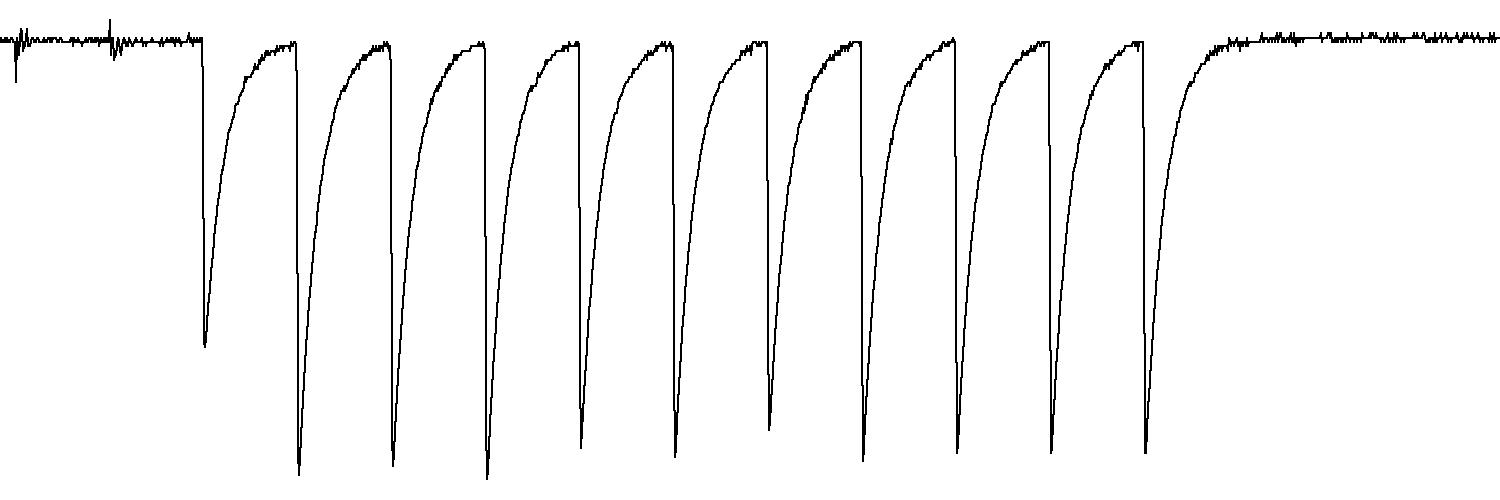
\includegraphics[width=0.9\textwidth]{./figures/power_trace/power_trace.png}
	\caption{SAKURA-G running AES, note its $10$ rounds. Data taken from \cite{exampletraces}.}
	\label{fig:powertrace}
\end{center}
\end{figure}

\subsubsection{Vulnerable Intermediate Result}
	
	In AES, the very first plaintext-dependent operation is $\AddRoundKey$ on Line~\ref{line:addrk} of Algorithm~\ref{alg:aes}, which XORs current state with the first block of expanded key. Here the state is equal to input plaintext, see Line~\ref{line:stateplain}, and the first block of expanded key is equal to the original AES key, see Note~\ref{note:expkey}. $\AddRoundKey$ is then usually composed with $\SubBytes$ (the following step), hence yielding
	\begin{equation}
	\label{eq:byprod}
		b = \SubBytes(k\xor m)
	\end{equation}
	as the first ($128$-bit wide) intermediate result, where $k$ stands for the AES key and $m$ for the plaintext. $b$ is then used in the following AES step which is $\ShiftRows$, usually composed with $\MixColumns$.
		
	Once we would learn $b$ and respective $m$ from a single AES encryption, it would be easy to directly compute the key as $k = {\SubBytes}^{-1}(b)\xor m$.

\subsubsection{Utilizing Power Traces}
	
	Yet in this attack scenario, we do not observe intermediate results $b$ directly, we only have power traces. Now let us describe a reasonable model how a certain portion of information about $b$'s leaks into the power trace, and how we can exploit it.
	
	Before entering next stages, the intermediate result $b$ is temporarily stored. It is handled byte-wise, hence its byte-wise Hamming weights (i.e., numbers of ones in binary representation, further denoted by $HW$) are reflected into the power trace\footnote{Here we assume the so-called {\em Hamming Weight Leakage Model}.}. It means that for each byte of $b$ denoted by $b_i$, there is a position in the power trace that reflects $HW(b_i)$.
	
	Let us suppose that we have a plenty of such traces which are properly aligned, i.e., a position in the traces corresponds with a fixed position in the AES implementation. Therefore, for each byte of $b$'s, there is a position in the traces, where the power values are correlated with Hamming weights of respective bytes of respective $b$'s.
	
	Since we do not know actual $b$'s, we will assume that the correlation of true values of $b$'s is the highest among others, and among all positions in the traces. Note that $b_i = S(k_i+m_i)$, i.e., $b$'s only depend on respective known plaintexts $m$ and the key $k$ which is constant, therefore we will loop through key guesses and search for globally maximal correlation. And more importantly, note that we can guess the key byte-wise!
	
	\begin{note}
	\label{note:brutevssca}
		In CPA we loop through $256$ key guesses for each of $16$ bytes, i.e., overall $256\cdot 16 = 2^{12} = 4096$ possibilities, compare with $256^{16} = 2^{128} = \ldots$ possibilities of a brute force attack.
	\end{note}

\subsubsection{Attack}
	
	The attack performs as follows: given a byte index $i=\atob{0}{15}$, we find the maximal correlation\footnote{We can rather use some other empirical meter, since correlation is quite expensive and we only need to find the key, no matter how.} (among all keyguesses $k_i$ of $i$-th byte of the key and all positions in the traces) of $HW\bigl(S(k_i+m_i)\bigr)$ with respective power values. $k_i$ reaching the maximum is then our top candidate. This idea is summarized in the following algorithm.
	
	\begin{alg}
	\label{alg:cpa}
	Given power traces and respective plaintexts, recover the AES key.
		\begin{algorithmic}[1]
			\Function{CPA\_Attack}{$Traces[N][T],PTs[N]$}
				\For{$i = 0 \to 15$}
					\State $max \gets 0$
					\For{$KGuess = \texttt{00} \to \texttt{ff}$}
						\State $tmpmax \gets \max\limits_{t\in T} \Corr\limits_{n\in N}\Bigl(Traces[n][t], HW\bigl(S(KGuess\xor PTs[n][i])\bigr)\Bigr)$
							\label{line:corr}
						\If{$tmpmax > max$}
							\State $max \gets tmpmax$
							\State $BestKey[i] \gets KGuess$
						\EndIf
					\EndFor
				\EndFor
				\State\Return $BestKey$
			\EndFunction
		\end{algorithmic}
	\end{alg}
	
	\begin{remark}
	\label{rem:attacklookup}
		We obviously do not compute SBox and Hamming weight at each step, but we rather use a single precomputed table of the composition of $HW\circ S$. Clearly, this table has $256$ entries in the range $\atob{0}{8}$.
	\end{remark}
	
	\begin{note}
	\label{note:fulllist}
		It is useful to modify the previous algorithm to output the whole list of key candidates together with their maximal correlation values for each key byte, i.e., the result of Line~\ref{line:corr}, not only $BestKey$.
		
		This is because if $BestKey$ is not equal to the true key, we still have a good chance to recover the key: since the true key is likely to have a rather high correlation, we loop through key candidates according to their correlation values -- in the descending order.
		
		Note that we can verify the correctness of our key guess simply by checking whether the resulting ciphertext equals to the ciphertext we expect.
	\end{note}
	
	\begin{note}
	\label{note:leakpos}
		It might be also helpful to output positions of maximal correlation for each candidate. This information might be valuable for any further analysis purposes.
	\end{note}
	
	There are several solutions implementing the CPA including the open-source ChipWhisperer\texttrademark\ Project \cite{chipwhisperer}, which is a toolkit providing a complete toolchain from trace acquisition to key extraction. We derived this algorithm from the ChipWhisperer\texttrademark documentation.


% ==============================================================================
% ===   B I T - W I S E   D P A                                              ===
% ==============================================================================

\subsection{Bit-Wise Differential Power Analysis Attack}

Let us continue with another attack on an unprotected AES implementation. For now, let us suppose a more powerful attacker, who can probe individual wires of a vulnerable bus and measure its voltage. Let us further suppose that the intermediate results $b = \SubBytes(k\xor m)$ are transferred over this bus.

Therefore such attacker is not limited to observing values related to the Hamming weight of $b$, but she can rather measure values related to individual bits of $b$! The advantage of such attacker is that there suffice much less measurements to successfuly recover the key.

\subsubsection{Attack}
	
	In this attack, we proceed similarly as in the previous one, i.e., we loop through key guesses for each key byte and compute the respective intermediate results $b_i$; see Algorithm~\ref{alg:cpa}. But instead of applying Hamming weight and computing correlation, we proceed with each bit individually.
	
	Let us say we are targetting the $j$-th bit of the $i$-th byte of $b$. Based on the actual key guess $k_i$, we compute the $j$-th bit of $b_i = S(k_i+m_i)$ for each trace/plaintext pair, and partition the traces based on this bit into two sets, let us denote them $S_0$ and $S_1$, respectively.
	
	\begin{note}
	\label{note:concattraces}
		Typically, we have several traces (from several probes) for a single plaintext and we do not know which of them contains which bit. Actually, this does not play much of a role -- we can serialize them into a single trace and do not care anymore.
	\end{note}
	
	If the key guess is correct, then there is a position in the traces, where the values are low in traces in $S_0$ and high in traces in $S_1$. We can find this position as the spot of the highest difference of mean values within $S_0$ and $S_1$. If the key guess is not correct, there should be no substantial peak in this difference of means. Hence the true key should maximize the trace-maximal difference of means among other key guesses. An algorithm implementing this attack follows.
	
	\begin{alg}
	\label{alg:bitwisedpa}
	Given voltage traces and respective plaintexts, recover the AES key.
		\begin{algorithmic}[1]
			\Function{Bitwise\_DPA\_Attack}{$Traces[N][T],PTs[N]$}
				\For{$i = 0 \to 15$}
					\State $max \gets 0$
					\For{$KGuess = \texttt{00} \to \texttt{ff}$}
						\For{$j = 0 \to 7$} \label{line:tbcycle}
							\State $S_0 \gets \Bigl\{ Traces[n] \Bigm| S\bigl(KGuess\xor PTs[n][i]\bigr)[j] = 0 \Bigr\}$ \label{line:s0}
							\State $S_1 \gets \Bigl\{ Traces[n] \Bigm| S\bigl(KGuess\xor PTs[n][i]\bigr)[j] = 1 \Bigr\}$ \label{line:s1}
							\State $tmpmax \gets \max\limits_{t\in T} \Bigl| \Mean\limits_{Trace\in S_1}\bigl(Trace[t]\bigr) - \Mean\limits_{Trace\in S_0}\bigl(Trace[t]\bigr) \Bigr|$
								\label{line:diffmean}
							\If{$tmpmax > max$}
								\State $max \gets tmpmax$
								\State $BestKey[i] \gets KGuess$
							\EndIf
						\EndFor
					\EndFor
				\EndFor
				\State\Return $BestKey$
			\EndFunction
		\end{algorithmic}
	\end{alg}
	
	\begin{note}
	\label{note:eightlists}
		We can modify this algorithm in a manner similar to Notes~\ref{note:fulllist} and \ref{note:leakpos}, and output the full record of maximal differences of means (instead of correlations previously, here it is the result of Line~\ref{line:diffmean}) and their positions in traces. Note that in this case we get $8$ separate lists for each $j$, see Line~\ref{line:tbcycle} in the previous algorithm. Here $j$ is referred to as the {\em target bit}. We can also unravel which target bit leaks most substantially, which might be useful for further analysis purposes.
	\end{note}
	
	To the best of our knowledge, there is no open-source project implementing this attack. This method has been taken from \cite{teuwen2015movfuscator}.
	

\section{Using SCA Tools in White-Box Attack Context}
\label{sec:scawbc}

%!% Bos et al. exploit leaked information instead, no need for exact knowledge of design nor reverse engineering
In the previous section, we presented some algorithms seemingly unrelated to what we have done so far. Indeed, our aim is to attack white-box implementations, where we can fully control the execution environment, thus there is no need for physical measurements. The actual reason emerges from a novel approach introduced recently by Bos et al.\ \cite{bos2015differential} -- the use of SCA tools in the context of white-box cryptography.

The idea was inspired by Delerabl{\'e}e et al.\ \cite{delerablee2013white}: as it is usually required, a ``perfect'' white-box implementation should not provide effectively any other information about the secret key, but only as much as an access to a black-box. Delerabl{\'e}e et al.\ observed that such implementation must be resistant to all existing and future side-channel attacks, which led Bos et al.\ to the idea of exploring this consequence by attacking white-box implementations with SCA tools. And the attack succeeded!

\begin{note}
\label{note:motiv}
	The previous observation also implies another motivation for white-box cryptography -- a white-box attack resistant implementation could be used for a SCA-resistant hardware implementation.
\end{note}

The obvious question is what kind of traces we should use instead of power traces -- we use {\em software traces}. In this context, software trace reffers to a record of memory addresses being accessed during program execution, or their contents; sometimes also referred to as {\em memory trace}. Hence in this context, differential power analysis might sound wierd, since there is no {\em power}, it will be rather referred to as {\em Differential Computation Analysis} (DCA).

In the following sections, we describe the full process of DCA attack -- from trace acquisition, over trace filtering, concluding with the attack itself.


% ==============================================================================
% ===   T R A C E   A C Q U I S I T I O N                                    ===
% ==============================================================================

\subsection{Trace Acquisition}
\label{sec:tracq}

In order to acquire a memory trace, we used Dynamic Binary Instrumentation (DBI) tools. These tools insert additional instructions to the original code of the program at run-time enabling one to debug or detect memory leaks. The most advanced DBI tools, like Valgrind \cite{nethercote2007valgrind} or PIN \cite{luk2005pin}, include a programmable interface, where one can write tools of own will. Both tools are open-source.

We modified a tool for PIN by Teuwen \cite{teuwen2015movfuscator} for $4$ use cases. These acquire
\begin{enumerate}
	\item addresses of memory reads, \label{item:readaddr}
	\item addresses of memory writes,
	\item contents of memory reads, and
	\item contents of memory writes, \label{item:writecnt}
\end{enumerate}
respectively. Tool nr.\ \ref{item:writecnt} is obviously most useful for unprotected implementations, since it can directly observe intermediate results, on the other hand, tool nr.\ \ref{item:readaddr} will be surprisingly used as well. The other tools will not be used in this thesis.

\begin{note}
\label{note:lsb}
	So far, we have not specified any possible limitations on memory traces. Note that in case we are catching addresses, we can limit our attention to the least significant byte only. Indeed, the rest of the address typically does not contain any relevant information, only the global position within memory, but the least significant byte carries information about the position within an array representing a WBAES table.
	
	In case of reading memory contents, we can only be interested in $1$-byte memory reads/writes, since AES tables are often constructed based on byte-wise representation.
\end{note}

Using chosen tool, we acquire certain amount of memory traces with different, possibly random, plaintexts on input. We save these plaintexts along corresponding traces, of course.

\begin{note}
\label{note:optim}
	In order to attack by SCA tools, traces must be properly aligned. It could happen that compiling C/C++ programs with high levels of optimization would produce misaligned traces -- we indeed experienced different lengths of traces.
	
	Therefore we recommend to compile C/C++ programs with different levels of optimization and acquire just a few traces for each level. We check traces' lengths and apply the highest optimization level, where the traces were equally long, and use this optimization level for trace acquisition.
\end{note}

One may wonder whether traces can ever be properly aligned, because then it would require additional effort to align them. According to our experience, traces were well aligned, hence there should be no need for this\footnote{Later we will introduce some countermeasures against this attack, including attempts to misalign traces. We will mention then another approach how we can treat trace misalignment.}.

\begin{note}
\label{note:aslr}
	There is another issue with trace acquisition, now it is related to the next step which is trace filtering. It will be highly appreciated that the program uses very the same addresses for instructions, which are not related to plaintext . Later we will try to filter them out, since they do not carry any useful information.
	
	For this reason it might be helpful to switch off Address Space Layout Randomization (ASLR) and acquire all traces in a single terminal session.
\end{note}

Having traces properly acquired, let us proceed to trace filtering.


% ==============================================================================
% ===   T R A C E   F I L T E R I N G                                        ===
% ==============================================================================

\subsection{Trace Filtering}
\label{sec:filter}

Once we have acquired memory traces, we perform two kinds of filtering. We filter trace entries
\begin{itemize}
	\item by constant value, and
	\item by address and temporal range.
\end{itemize}

\subsubsection{Filtering of Constant Entries}
	
	In the first stage, we filter out such entries which are constant across all acquired traces, because they do not carry any information. Indeed, both presented SCA algorithms exploit changes across traces.
	
	Practically, we first create a filter mask based on a small subset of traces, $10$ appears to be sufficient. Such mask carries $0$ if all corresponding addresses in the small set of traces are equal, $1$ otherwise; see an example in Figure \ref{fig:constmask}. This mask is then simply applied to filter all the remaining traces, possibly hundreds or thousands of them. Note that we keep the mask, we will use it for the following filtering method as well.
	
	\begin{figure}[H]
	\[
	\arraycolsep=.5em\def\arraystretch{1.5}
		\begin{array}{|c|ccccccccc|}
			\hline
			\textnormal{Trace 0} & {\tt 65} & {\tt de} & {\tt 37} & {\tt 7e} & {\tt 63} & {\tt 30} & {\tt c0} & {\tt 62} & {\tt 61} \\
			\textnormal{Trace 1} & {\tt 65} & {\tt de} & {\tt 31} & {\tt 7e} & {\tt 23} & {\tt 30} & {\tt b1} & {\tt 62} & {\tt 61} \\
			\textnormal{Trace 2} & {\tt 65} & {\tt de} & {\tt 1f} & {\tt 7e} & {\tt d5} & {\tt 30} & {\tt 77} & {\tt 62} & {\tt 61} \\
			\textnormal{Trace 3} & {\tt 65} & {\tt de} & {\tt 97} & {\tt 7e} & {\tt 5c} & {\tt 30} & {\tt c4} & {\tt 62} & {\tt 61} \\
			\hline
			\textnormal{Mask}    & {\tt 0}  & {\tt 0}  & {\tt 1}  & {\tt 0}  & {\tt 1}  & {\tt 0}  & {\tt 1}  & {\tt 0}  & {\tt 0} \\
			\hline
		\end{array}
	\]
	\caption{An example of a mask used for trace filtering.}
	\label{fig:constmask}
	\end{figure}
	
	\begin{note}
	\label{note:filter}
		Filtering of constant entries typically decreases the size of the traces by tens of percent. If we did not observe any or extremely small decrease, it might have happened that the traces were not properly aligned. In such case, it might be difficult to align them. Fortunately, we did not experience this problem (we gave some advices how to avoid it in Note \ref{note:aslr}).
	\end{note}

\subsubsection{Address and Temporal Filtering}
\label{subsec:atf}
	
	In the second stage, we will filter the traces based on visual observation. Note that for this purpose, we will need to acquire another trace with full read/write addresses for all types of memory traces, unlike Note \ref{note:lsb}. We will refer to such trace as {\em full trace}.
	
	We will proceed as follows: first we acquire a full trace and filter it by the mask from the previous method. Then we visualize it and try to find out, in which address and temporal range encryption takes place. Based on our observation, we filter our traces using this range.
	
	\begin{note}
	\label{note:fullfilter}
		Once we filter the full trace, we get rid of tons of ballast yielding a trace which is much smaller and easier to understand. Note that the filtered full trace remains correctly aligned to the rest of our traces after filtering.
	\end{note}
	
	\paragraph{Trace Visualization}
		
		We developed a primitive tool displaying a full memory trace for this purpose. Given $n$ and a trace, this tool splits the trace by addresses into $n$ ``compact'' segments and displays these parts separately. See Figure \ref{fig:memtrace} for an illustrative memory trace of a run of a simple AES implementation. Horizontal axis represents address range, vertical axis represents temporal range (from the top).
		
		\begin{figure}[h!]
		\begin{center}
			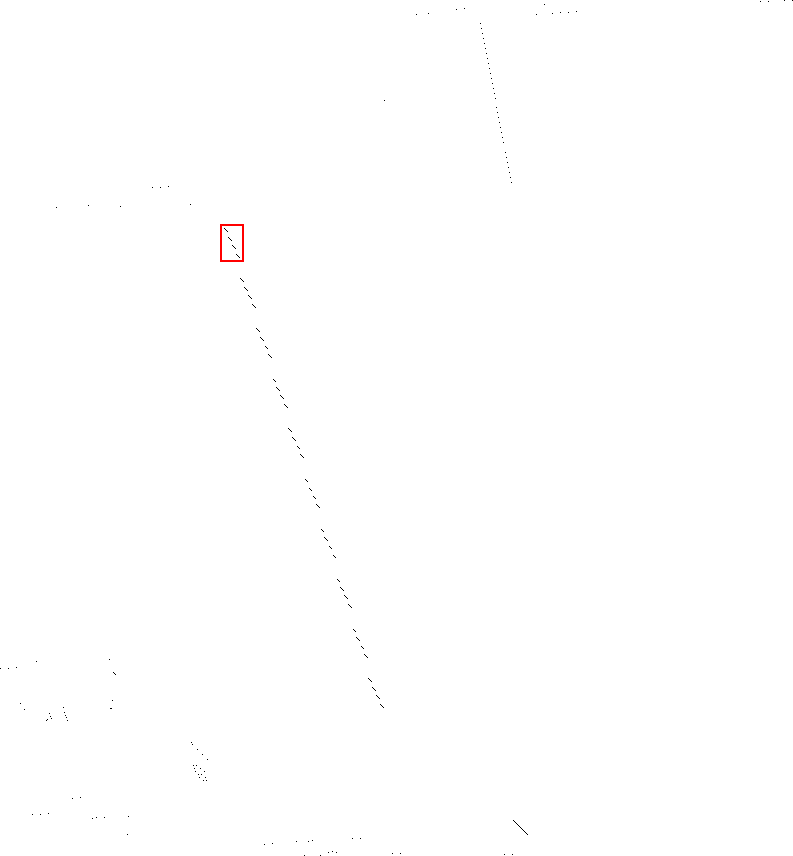
\includegraphics[width=0.9\textwidth]{./figures/memtrace/memtrace_emph.png}
			\caption{Illustrative memory trace of a run of a simple AES implementation with the first round emphasized by a red rectangle. Contents of memory writes were acquired.}
			\label{fig:memtrace}
		\end{center}
		\end{figure}
		
		In this example trace, we can clearly recoginze $10$ distinct AES rounds even with its $4$ subroutines. In general, if possible, we try to estimate the address and temporal range of the first round\footnote{Note that we are only interested in the first round, see Equation \ref{eq:byprod} and its context.} based on visual observation. In the example, the first round is emphasized by a red rectangle.

	\paragraph{Trace Filtering}
		
		Given an address and temporal range, we filter our traces so that we only keep their entries which fall into this range. But our traces do not contain full address information, see Note \ref{note:lsb}. The idea could be to use full traces instead.
		
		If we had all full traces, we could filter them easily based on both ranges. But in this case there may occur a position, for which some traces contain an address falling inside or outside the address range, respectively. Note that this would immediately violate the alignment!
		
		\begin{remark}
		\label{rem:rangemask}
			There is a better way how to filter our traces by address and temporal range. We simply take our single filtered full trace and create another mask, see Example \ref{ex:rangemask}. Then we filter our traces with this mask as we did before. This approach ensures that the traces keep aligned.
		\end{remark}
		
		\begin{example}
		\label{ex:rangemask}
			Let say we have deduced from trace visualization that the first round of AES encryption takes place between rows $0$ and $2$, and in the address range from {\tt 0x7fffe3150000} to {\tt 0x7fffe3158000}. Then we get the mask as follows.
			\[
			\arraycolsep=.5em\def\arraystretch{1.5}
				\begin{array}{|c|c|c|}
					\hline
					\textnormal{Row} & \textnormal{Filtered Full Trace} & \textnormal{Mask} \\
					\hline
					0 & {\tt 0x7fffe314f028} & {\tt 0} \\
					1 & {\tt 0x7fffe3150ac8} & {\tt 1} \\
					2 & {\tt 0x7fffe3151dc8} & {\tt 1} \\
					3 & {\tt 0x7fffe3152d18} & {\tt 0} \\
					4 & {\tt 0x7fffe3153948} & {\tt 0} \\
					\hline
				\end{array}
			\]
		\end{example}
		
		Note that address and temporal filtering brings the most substantial speedup of the whole attack, since its speed depends heavily on the size of the traces. On the other hand, it may happen that we filter our traces too much and loose valuable information, i.e.\ the attack does not succeed. In such case, we broaden the address and/or temporal range and rerun again.
		
		Also note that there may occur several $10$-part patterns resembling $10$ AES rounds. Then we need to keep trying them all until we succeed with our attack.
		
		In the worst case, all our filtering attempts fail or we just cannot see any relevant pattern in the memory trace visualization. Then we omit address and temporal filtering at all and attack for instance only the first byte while, hopefuly, obtaining the position where the key leaks, i.e.\ where encryption takes place; here we employ the improved output of our SCA algorithm introduced in Note \ref{note:leakpos}. We can look at this position in the visualization and guess some reasonable address and temporal range, use it for filtering and finally attack all $16$ bytes with much smaller traces.


% ==============================================================================
% ===   A T T A C K I N G   T R A C E S                                      ===
% ==============================================================================

\subsection{Attacking Traces}
\label{sec:attack}

Once the traces are acquired, possibly filtered and, most importantly, properly aligned -- it can be deduced from Note \ref{note:filter} and achieved with ideas from Note \ref{note:aslr} --, we can perform the attack. We can use both SCA algorithms presented in this thesis, i.e.\ Algorithm \ref{alg:cpa} or \ref{alg:bitwisedpa}, or any other SCA algorithm of our choice.

\begin{remark}
\label{rem:traceformat}
	Remind that each of our two SCA algorithms was originally designed for a different kind of traces.
	
	In Algorithm \ref{alg:cpa}, the traces were supposed to carry information about Hamming weight of intermediate results, therefore the original attack must be modified to compute Hamming weights of entries of traces. It might not make much sense to compute Hamming weight of both intermediate result and trace entries and then their correlation, but this algorithm serves rather as a proof-of-concept. On the other hand, it could possibly bring some surprising results, so we employed it as well.
	
	In Algorithm \ref{alg:bitwisedpa}, the traces were supposed to be a serialization of eight separate traces, which should carry only bits of information; see Note \ref{note:concattraces}. Therefore it is crucial in this attack to consider entries of traces as separate bits, not bytes, i.e.\ {\tt [1,0,0,0,0,1,0,0, 0,1,1,0,1,1,0,0]} rather than {\tt [84, 6c]}.
\end{remark}

As outlined in the previous remark, we will consider Algorithm \ref{alg:bitwisedpa} by default since now, unless stated otherwise.

\subsubsection{Processing Results}
	
	As already stated in Note \ref{note:fulllist}, the best key candidate we obtain from a SCA algorithm does not need to be necessarily the correct one, especially when we use it for attacking white-box implementations, where there is no interpretation of what we ``measure''.
	
	In that note, we suggested to output the full list of key candidates together with their ``value'' for each key byte. The original purpose of this was to have some rating of key candidates, and then loop through them according to their order and value. In physical world scenario, this would be likely to recover the key in a relatively short time, since we assume certain bias in our measurements caused by execution of the cipher.
	% \footnote{Each SCA algorithm may use different meter to compare key candidates, in Algorithm \ref{alg:cpa} it was correlation, in Algorithm \ref{alg:bitwisedpa} it was difference of means.}
	
	But it turns out that looping would be useless in the white-box scenario. Indeed, by empirical observation, the true key byte is typically
	\begin{itemize}
		\item either on the top separated by a gap from the second candidate, or
		\item somewhere in between while the first candidate is separated by a smaller gap,
	\end{itemize}
	see the following example with real data. This observation is especially useful for our $8$ separate lists; see Note \ref{note:eightlists}.
	
	\begin{example}
	\label{ex:gap}
	See the following table for partial results of a real experiment, find further comments below.
		\begin{table}[H]
			\begin{center}
			\begin{tabular}{| c | c | c | c | c | c | c | c | c |}
				\hline
				\multirow{2}{*}{Rank} & \multicolumn{2}{c|}{\nth{4} bit} & \multicolumn{2}{c|}{\nth{5} bit} & \multicolumn{2}{c|}{\nth{7} bit} & \multicolumn{2}{c|}{\nth{8} bit} \\
				\cline{2-9}
					~ & Value & Cand.   & Value & Cand.   & Value & Cand.   & Value & Cand.  \\
				\hline
					0      & 0.3477 & {\tt >15<} & 0.3970 & {\tt 09}   & 0.3374 & {\tt 9d}   & 0.3730 & {\tt 6f}   \\
					1      & 0.3147 & {\tt b5}   & 0.3884 & {\tt d1}   & 0.3196 & {\tt f5}   & 0.3521 & {\tt 8b}   \\
					2      & 0.3110 & {\tt e7}   & 0.3699 & {\tt 65}   & 0.3183 & {\tt 37}   & 0.3451 & {\tt 7b}   \\
					\vdots & \vdots & \vdots     & \vdots & \vdots     & \vdots & \vdots     & \vdots & \vdots     \\
					23     & \vdots & \vdots     & \vdots & \vdots     & 0.2895 & {\tt fc}   & \vdots & \vdots     \\
					24     & \vdots & \vdots     & \vdots & \vdots     & 0.2892 & {\tt >15<} & \vdots & \vdots     \\
					25     & \vdots & \vdots     & \vdots & \vdots     & 0.2890 & {\tt df}   & \vdots & \vdots     \\
					\vdots & \vdots & \vdots     & \vdots & \vdots     & \vdots & \vdots     & \vdots & \vdots     \\
					41     & \vdots & \vdots     & \vdots & \vdots     & \vdots & \vdots     & 0.2840 & {\tt c1}   \\
					42     & \vdots & \vdots     & \vdots & \vdots     & \vdots & \vdots     & 0.2838 & {\tt >15<} \\
					43     & \vdots & \vdots     & \vdots & \vdots     & \vdots & \vdots     & 0.2825 & {\tt b8}   \\
					44     & \vdots & \vdots     & 0.2760 & {\tt be}   & \vdots & \vdots     & \vdots & \vdots     \\
					45     & \vdots & \vdots     & 0.2760 & {\tt >15<} & \vdots & \vdots     & \vdots & \vdots     \\
					46     & \vdots & \vdots     & 0.2759 & {\tt c4}   & \vdots & \vdots     & \vdots & \vdots     \\
					\vdots & \vdots & \vdots     & \vdots & \vdots     & \vdots & \vdots     & \vdots & \vdots     \\
				\hline
			\end{tabular}
			\end{center}
		\caption{Partial results of a real experiment. The true key byte is {\tt 15} and is emphasized with angle brackets.}
		\label{tab:gap}
		\end{table}
		According to the original criterion, i.e.\ picking the candidate with the highest value, we would get {\tt 09} in the \nth{5} bit column, but it is not the correct one -- in this experiment, the true candidate does not have the highest value.
		
		On the other hand, if we consider the gap to the second candidate and modify our criterion to take it into account, we can get the correct candidate.
	\end{example}
	
	\begin{remark}
	\label{rem:gap}
		According to the observation in the previous example, we can modify our criterion as follows: we choose the candidate which is on the top of any list and has the biggest gap to the second candidate. Note that we can use various methods how to evaluate this gap, e.g.\ absolute or relative differences of values, and we may obtain different results.
		
		We can further improve this rule by combining (e.g.\ summing) gaps of the same candidate when it is on the top. On the other hand, note that if the correct candidate is not on the top of any list, improving this rule does not help either.
		
		Similarly to the idea of Note \ref{note:fulllist}, we can create a list of maximum $8$ candidates (one candidate from each of $8$ lists) and loop through them to find out whether the key was revealed or not.
	\end{remark}
	
	Applying the rule from the previous remark to the previous example, we find the maximal gap for the \nth{4} target bit, its absolute value is $0.0330$ compared to $0.0086$, $0.0178$ and $0.0209$, its relative value is $9.5\%$ compared to $2.2\%$, $5.3\%$ and $5.6\%$, respectively. Hence the best candidate with this rule is {\tt 15} which is the correct one.
	
	\begin{note}
	\label{note:strong}
		For later use, we recognize two kinds of best candidates according to the gap to the second candidate. If the gap is greater than $10\%$, it will be referred to as {\em strong candidate}, otherwise it will be referred to as {\em weak candidate}.
	\end{note}

		
		%%% KAPITOLA 3
		\chapter{Results \& Improvements}
\label{chap:results}

%!% blbiny ...
First we describe what tools we needed to perform a practical attack, then we present and discuss our results. Finally we outline possible enhancements of the attack and present our contribution.

\section{Attack Tools}
\label{sec:tools}

Since there is no open-source toolkit\footnote{At the time of writing. However, it should be available soon from the original authors.} for the purpose of DCA described in Section \ref{sec:scawbc}, we implemented it ourselves. Our toolkit consists of several tools and subtools, see the following list.

%!% vočekovat, Teuwen psal mail že to brzy uvolní jako open-source

\begin{itemize}
	\item Acquire traces (see Section \ref{sec:tracq}):
	\begin{itemize}
		\item acquire single trace (PIN tools, modified versions of Teuwen's one \cite{teuwen2015movfuscator}),
		\begin{itemize}
			\item memory reads/writes and their addresses/contents,
		\end{itemize}
		\item manage trace acquisition (generate \& save respective plaintexts along).
	\end{itemize}
	\item Filter traces (see Section \ref{sec:filter}):
	\begin{itemize}
		\item filter constant entries \& save its mask $M_C$ (see Figure \ref{fig:constmask}),
		\item filter by address and temporal range,
		\begin{itemize}
			\item acquire another {\em full} trace $T$ (preferably in the same terminal session),
			\item filter it with mask $M_C$ yielding $T_C$,
			\item visualize $T_C$,
			\item estimate address \& temporal range,
			\item create another mask $M_R$ based on the range using $T_C$,
			\item filter all traces with $M_R$ (see Remark \ref{rem:rangemask}).
		\end{itemize}
	\end{itemize}
	\item Attack traces (see Section \ref{sec:attack}):
	\begin{itemize}
		\item run attack,
		\begin{itemize}
			\item CPA attack (Algorithm \ref{alg:cpa}), or
			\item bit-wise DPA attack (Algorithm \ref{alg:bitwisedpa}),
		\end{itemize}
		\item process \& display results.
	\end{itemize}
\end{itemize}


\section{Results}
\label{sec:results}

First we used our toolkit to attack our straightforward implementation of AES, here named {\tt naiveAES}, which served just as a proof-of-concept. Then we performed the most interesting attack which Bos et al. \cite{bos2015differential} did -- we successfuly attacked Klinec's implementation \cite{klinec2013implementation} of WBAES by Chow et al. \cite{chow2003aes}, here named {\tt KlinecWBAES}.

Note that the following Section \ref{sec:naiveaes} giving results of attack against {\tt naiveAES} does not fully cover many details, these are given separately in the subsequent Section \ref{sec:klinecwbaes} with results of attack against {\tt KlinecWBAES}.


% ======================================================================
% ===   n a i v e A E S                                              ===
% ======================================================================

\subsection{\tt naiveAES}
\label{sec:naiveaes}

In order to prove the concept of both SCA algorithms presented in this thesis, we first attacked our straightforward AES implementation {\tt naiveAES} with both of them.

\subsubsection{CPA against {\tt naiveAES}}
	
	We repeated CPA attack (i.e. Algorithm \ref{alg:cpa}) with $10$ different keys and for different amounts of plaintexts. See results in Table \ref{tab:naiveaes}.
	
	\begin{table}[H]
		\begin{center}
		\begin{tabular}{| c | c | c | c |}
			\hline
			~ & \multicolumn{2}{c|}{\bf $n\times n$ squares} & {\bf Computational} \\
			~ & \multicolumn{1}{c}{Lower bound} & \multicolumn{1}{c|}{Upper bound} & {\bf Power}\\
			\hline
			2D & \multicolumn{2}{c|}{See see} & Universal \\
			\hline
			2D & see & see & Unknown \\
			\hline
		\end{tabular}
		\end{center}
	\caption{CPA against }
	\label{tab:naiveaes}
	\end{table}

\subsubsection{Bit-Wise DPA against {\tt naiveAES}}
	
	Algorithm \ref{alg:bitwisedpa}
	
	%?% vyzkoušet rijinv na naiveAES, nemělo by jít


% ======================================================================
% ===   K l i n e c W B A E S                                        ===
% ======================================================================

\subsection{\tt KlinecWBAES}
\label{sec:klinecwbaes}



%~ co jsem použil za implmentace, kolik traců, jak dlouho to běželo, že jsem zjistil adresu kde to leakuje
%~ teoreticky by mělo bejt popsáno v předch. kapitole, tady už bych jenom zmínil co jsem použil a co vypadlo
%~ a proč to s tou javou nešlo ... (ale vyzkoušet)
%~ de facto takovej protokol
%~ Two (?) implementations will be considered for the attack:
%~ \begin{itemize}
	%~ \item our naive AES implementation (C++), and
	%~ \item Klinec's implementation of White-Box AES \cite{klinec2013white} (C++).
%~ \end{itemize}
%~ NaiveAES implementation was broken by both algorithms, CPA attack required $x$ traces, bitwise DPA attack required $y$ traces.
%~ White-Box-AES implementation was only broken by bitwise DPA attack and many interesting things occured.
% provést útok s několikrát nagenerovanejma tabulkama (v manuálu pak popsat co je pro to potřeba udělat)



\section{Enhancements of the Attack}   %?% to/of ?
\label{sec:enhancements}

%~ Before we introduce our improvements, we present one of Bos et al.\ \cite{bos2015differential} and reproduce their results in order to have some comparison of our method with previous results.
In this section we propose our novel improvement of the attack and present its practical results. But before we do so, we introduce an enhancement by Bos et al.\ \cite{bos2015differential} and reproduce their results in order to have some comparison with previous results for our method.
%~ We will later use these reproduced results for comparison with our novel approach.
%~ We will later use these reproduced results as a reference for our novel approach.


% ==============================================================================
% ===   E X P L O I T I N G   W B A E S   S T R U C T U R E                  ===
% ==============================================================================

\subsection{Exploiting WBAES Structure}

WBAES by Chow et al.\ \cite{chow2002aes} has been shown by Klinec \cite{klinec2013white} to be eqivalent to Karroumi's improved version \cite{karroumi2011protecting}. Remind that Karroumi's WBAES uses internally dual AES'es and therefore we cannot recognize which affine mapping has been used inside SBoxes, see Note \ref{note:dualsbox}.

Let us first remind definition of the original SBox (Equation \ref{eq:sbox}) and also remind that the multiplication is not performed in $F$, but in the ring of binary polynomials instead:
\[
	\defsbox .
\]
Note that the original SBox is a specific affine mapping of Rijndael inverse of its input while in Karroumi's approach, this affine mapping is not fixed. Such a new SBox could be written as   %?% neni už to dopsaný tam dřív?
\begin{equation}
\label{eq:spq}
	S_{p,q}(A) = p\cdot A' + q \pmod{x^8+1}
\end{equation}
for $p,q\in F$ and $p$ coprime with $x^8+1$. The simplest affine mapping is obviously achieved for $p=1$ and $q=0$ which yields $S_{1,0}(A) = A'$ i.e.\ only a Rijndael inverse.

\begin{remark}
\label{rem:coprime}
	The reason why $p$ must be coprime with $x^8+1$ was already given in the definition of the original SBox in Note \ref{note:sboxinv} -- it was due to its invertibility. Hence we would like to test whether $p$ is coprime with $x^8+1$.
	
	Note that $x^8+1 = (x+1)^8$, therefore if $p$ is {\em not} coprime with $x^8+1$, then $1$ must be its root, and vice versa. This can be easily tested, indeed $p(1) = 0$ if the number of its terms is even. It follows that $p$ is coprime with $x^8+1$ if and only if the number of terms of $p$ is odd.
\end{remark}


% ==============================================================================
% ===   C H A N G I N G   A T T A C K   T A R G E T                          ===
% ==============================================================================

\subsection{Changing Attack Target}
\label{sec:rijinv}

Since all of these SBoxes are equivalent inside WBAES, Bos et al.\ came up with the idea of changing the target of the attack from the original SBox to its simplest variant -- Rijndael inverse.

\begin{remark}
\label{rem:spq}
	Technically we only substitute SBoxes on Line \ref{line:s0} and \ref{line:s1} of Algorithm \ref{alg:bitwisedpa} with their desired variant, hence yielding
	\begin{align}
	\begin{split}
	\label{eq:target}
		S_0 &\gets \Bigl\{ Traces[n] \Bigm| S_{1,0}\bigl(KGuess\xor PTs[n][i]\bigr)[j] = 0 \Bigr\} , \\
		S_1 &\gets \Bigl\{ Traces[n] \Bigm| S_{1,0}\bigl(KGuess\xor PTs[n][i]\bigr)[j] = 1 \Bigr\} .
	\end{split}
	\end{align}
	Remind that we always use precomputed SBox tables as already stated in Remark \ref{rem:attacklookup}.
\end{remark}

\begin{note}
\label{note:target}
	The term {\em target of the attack} or simply {\em target} will be used heavily in the following text, let us describe it a bit closer.
	
	Target is a function $T$ which inputs a key byte $K$ together with a respective plaintext byte $P$ and outputs a byte (for now) or a single bit (later), e.g.\ $T(K,P) = S_{1,0}(K\xor P)$ (cf.\ Equations \ref{eq:target}). Target bit is just a specific bit of target's output. According to the target bit, traces are split into the sets $S_0$ and $S_1$ in Algorithm \ref{alg:bitwisedpa}, respectively.
\end{note}

\subsubsection{Results using Rijndael Inverse}
	
	We conducted the same attack as in Section \ref{sec:klinecwbaes}, now with Rijndael inverse as the target (i.e.\ the simplest SBox variant), see results in Table \ref{tab:klinecrijinv}. Note that this is the second part of successfuly reproduced results of Bos et al.
	
	\afterpage{
		\clearpage   % To flush out all floats, might not be what you want
		\begin{landscape}
		\begin{table}[H]
			\begin{center}
			\begin{tabular}{| c | r@{.} l@{\quad}r | r@{.} l@{\quad}r | r@{.} l@{\quad}r | r@{.} l@{\quad}r | r@{.} l@{\quad}r | r@{.} l@{\quad}r | r@{.} l@{\quad}r | r@{.} l@{\quad}r |}
	\hline
	\multirow{2}{*}{Byte} & \multicolumn{24}{c|}{Target bits (percentual gap\quad rank)} \\
	\cline{2-25}
	~ & \multicolumn{3}{c|}{1. bit} & \multicolumn{3}{c|}{2. bit} & \multicolumn{3}{c|}{3. bit} & \multicolumn{3}{c|}{4. bit} & \multicolumn{3}{c|}{5. bit} & \multicolumn{3}{c|}{6. bit} & \multicolumn{3}{c|}{7. bit} & \multicolumn{3}{c|}{8. bit} \\
	\hline
	\hline
	1.&3&3&207&45&4&{$\blacksquare$}&9&4&4&7&4&252&2&6&253&11&0&252&43&6&{$\blacksquare$}&35&3&{$\blacksquare$}\\
	\hline
	2.&5&4&233&1&3&255&0&9&252&49&4&{$\blacksquare$}&4&1&216&8&6&255&10&6&255&47&9&{$\blacksquare$}\\
	\hline
	3.&0&5&254&9&5&209&20&6&{$\blacksquare$}&45&6&{$\blacksquare$}&7&0&254&0&4&225&8&9&247&2&8&189\\
	\hline
	4.&2&1&37&12&7&{$\blacksquare$}&10&7&251&2&0&{\weak$\blacksquare$}&7&2&{\weak$\blacksquare$}&4&9&252&0&7&231&9&0&242\\
	\hline
	5.&2&1&244&17&9&{$\blacksquare$}&5&7&250&0&4&231&2&5&134&2&0&79&5&8&214&3&6&223\\
	\hline
	6.&53&2&{$\blacksquare$}&1&3&253&8&9&255&9&0&254&38&2&{$\blacksquare$}&37&8&{$\blacksquare$}&43&6&{$\blacksquare$}&7&3&2\\
	\hline
	7.&24&5&{$\blacksquare$}&0&9&248&6&4&187&5&8&255&13&6&209&36&2&{$\blacksquare$}&0&9&184&2&7&227\\
	\hline
	8.&48&9&{$\blacksquare$}&7&4&255&4&2&255&6&5&242&8&1&234&1&9&253&47&2&{$\blacksquare$}&2&8&255\\
	\hline
	9.&0&3&227&0&6&156&6&0&237&2&5&243&14&4&229&6&2&232&51&3&{$\blacksquare$}&15&1&{$\blacksquare$}\\
	\hline
	10.&8&9&{\weak$\blacksquare$}&3&0&158&10&1&1&40&5&{$\blacksquare$}&4&2&253&12&2&{$\blacksquare$}&54&3&{$\blacksquare$}&50&1&{$\blacksquare$}\\
	\hline
	11.&4&7&248&51&7&{$\blacksquare$}&6&7&241&0&4&254&4&4&251&5&2&45&10&1&255&4&7&1\\
	\hline
	12.&43&2&{$\blacksquare$}&2&8&251&7&2&254&2&5&255&6&9&236&3&2&255&49&2&{$\blacksquare$}&6&2&254\\
	\hline
	13.&7&3&205&6&2&4&9&2&191&6&6&30&63&7&{$\blacksquare$}&14&7&{$\blacksquare$}&7&5&240&0&8&255\\
	\hline
	14.&61&4&{$\blacksquare$}&4&9&231&1&7&246&54&4&{$\blacksquare$}&1&9&248&9&7&253&15&8&{$\blacksquare$}&46&2&{$\blacksquare$}\\
	\hline
	15.&0&7&221&2&0&250&4&7&1&2&0&{\weak$\blacksquare$}&8&0&223&31&3&{$\blacksquare$}&1&4&1&21&0&225\\
	\hline
	16.&4&0&255&57&7&{$\blacksquare$}&6&5&229&4&3&254&47&1&{$\blacksquare$}&9&5&255&8&2&254&1&7&253\\
	\hline
\end{tabular}   %!% obrátit pořadí sloupečků !!!
			\end{center}
		\caption{Bit-Wise DPA attack against {\tt KlinecWBAES} using $1024$ traces, Rijndael inverse taken as the target.}
		\label{tab:klinecrijinv}
		\end{table}
		\end{landscape}
	}
	
	On average, there are about $27\%$ of successful strong candidates and about $30\%$ of both weak and strong ones.
	
	In both cases (i.e.\ Table \ref{tab:klinecsbox} and \ref{tab:klinecrijinv}), there are, for each key byte, usually either only few target bits which actually leak, or nothing leaks at all (e.g.\ \nth{9} byte in Table \ref{tab:klinecsbox} cannot be considered as leaking, since the gap is very small at \nth{7} bit and at \nth{8} bit, the gap is much larger for an incorrect candidate; this happens much more often if less traces are used).
	
	The most substantial practical benefit of attacking different targets is that those key bytes, which did not leak with one target, may possibly leak with another, cf. \nth{9} byte in both tables.


% ==============================================================================
% ===   C O N S I D E R I N G   A N O T H E R   T A R G E T S                ===
% ==============================================================================

\subsection{Considering Another Targets}
\label{sec:16targets}

The benefit of having higher chance of breaking the key led us to the idea of using yet another invertible affine mappings inside SBoxes (see Equation \ref{eq:spq}) besides the one of the original SBox and identity (i.e.\ those used by Bos et al.).

There seems to be plenty of them: number of $p$'s is equal to the number of binary polynomials with degree smaller than $8$ which are coprime with $x^8+1$, there are $128$ of them (follows from Remark \ref{rem:coprime}). Number of $q$'s is simply $256$, hence altogether there are $128\cdot 256 = 32\,768$ invertible affine mappings which could be used inside SBoxes to create another targets.

\newpage   %!% zmrd bez toho píčuje

\begin{remark}
\label{rem:pqeffect}
	We realized that there are certain classes of mappings which give very the same results.
	\begin{description}
		\item[Effect of $q$'s.]
			First let us see what happens if we change one bit of $q$ (here considered as a byte). It obviously only changes the output of our SBox at the same bit, finally yielding a swap of $S_0$ and $S_1$ in the attack algorithm (only at this target bit, of course). Note that this swap has no effect on results, since we are only interested in absolute difference of means of values inside $S_0$ and $S_1$. Hence we will consider $q = 0$, our SBoxes will then be linear mappings of Rijndael inverse.
		
		\item[Effect of $p$'s.]
			Second let us study the effect of different $p$'s. Note that $x$ is coprime with $x^8+1$ and $p$ is supposed to be coprime, too, therefore if we multiply $p$ by $x\pmod{x^8+1}$, the result is still coprime with $x^8+1$.
			
			Now let us see what multiplying by $x\pmod{x^8+1}$ actually does. If the result does not need to be reduced, it simply shifts coefficients of $p$ by one, e.g.\ $(x^4 + x + 1) \cdot x = x^5 + x^2 + x$. If it reaches $x^8$, e.g.\ $(x^7 + x^4 + x^3) \cdot x \pmod{x^8+1} = x^5 + x^4 + 1$, we get $1$ at the end so the shift is actually a cyclical shift.
			
			Remind that polynomials, which are coprime with $x^8+1$, have odd number of terms (see Remark \ref{rem:coprime}), hence repeating multiplication by $x$ yields $8$ distinct polynomials which we put in single equivalence class. Since there are $128$ coprime polynomials, we get $128/8=16$ such classes, see Table \ref{tab:classrepre} for representants of each class. Note that the effect is the same on bits representing polynomials.
			
			Since we assumed $q = 0$, the actual output of two SBoxes using $p$'s from single class is thus also only a cyclical shift of each other. It follows that the effect on results is only a cyclical shift of the results among target bits. Hence also the information which target bit leaks is totally irrelevant.
	%?% neni zas tak irelevant ptž z pozice v trace zjistim která varianta to je, ze všech mi to pak může něco prozradit
	% => je irrelevant ptž ikdyž leaknou dva tak rozhodně nejsou od sebe jak by měly
	\end{description}
\end{remark}

\begin{table}[h]
	\begin{center}
	\begin{tabular}{| c | c | c | c | c | c | c | c |}
		\hline
		{\tt 01} & {\tt 07} & {\tt 0b} & {\tt 0d} & {\tt 13} & {\tt 15} & {\tt 19} & {\tt 1f} \\
		\hline
		{\tt 25} & {\tt 2f} & {\tt 37} & {\tt 3b} & {\tt 3d} & {\tt 57} & {\tt 5b} & {\tt 7f} \\
		\hline
	\end{tabular}
	\end{center}
\caption{Representants of classes of $p$'s in hexadecimal form. Remind that $p$ of the original SBox is {\tt 1f}.}
\label{tab:classrepre}
\end{table}

It follows that we can narrow down our attention to $16$ targets only. Indeed, our targets will be of the form $T(K,P) = S_{p,0}(K\xor P)$ for all representants $p$, see Table \ref{tab:classrepre}. Remind that Bos et al.\ only used the original SBox (i.e.\ $p = \texttt{1f}$) and Rijndael inverse (i.e.\ $p = \texttt{01}$).


% ==============================================================================
% ===   A T T A C K   U S I N G   A L L   1 6   T A R G E T S                ===
% ==============================================================================

\subsection{Attack Using All 16 Targets}

We attacked {\tt KlinecWBAES} using all of the $16$ attack targets and $1024$ traces, see results of the \nth{1} byte in Table \ref{tab:lintargets}. Note that the row of target {\tt 01} is indeed equal to the row of the \nth{1} byte in Table \ref{tab:klinecrijinv} and the row of target {\tt 1f} is indeed equal to the row of the \nth{1} byte in Table \ref{tab:klinecsbox}. Also note that the target {\tt 25} does not unravel the \nth{1} key byte even with $1024$ traces -- here we can clearly see the benefit of having many targets.

\afterpage{
	\clearpage   % To flush out all floats, might not be what you want
	\begin{landscape}
	\begin{table}[H]
		\begin{center}
		\begin{tabular}{| c | l@{\;} r@{.}l | l@{\;} r@{.}l | l@{\;} r@{.}l | l@{\;} r@{.}l | l@{\;} r@{.}l | l@{\;} r@{.}l | l@{\;} r@{.}l | l@{\;} r@{.}l |}
	\hline
	Tg. & \multicolumn{24}{c|}{Target bits} \\
	\hline
	{\tt 01}&\quad&0&15&$\square$&17&72&\quad&6&93&\quad&4&65&\quad&5&37&\quad&1&07&$\square$&13&48&$\blacksquare$&25&72\\
	\hline
	{\tt 07}&\quad&5&24&\quad&8&67&\quad&4&06&$\blacksquare$&47&88&\quad&8&15&$\square$&25&40&\quad&0&32&\quad&3&87\\
	\hline
	{\tt 0b}&$\square$&0&16&\quad&2&73&\quad&0&19&\quad&1&60&\quad&0&28&\quad&4&03&$\square$&18&07&$\blacksquare$&45&42\\
	\hline
	{\tt 0d}&$\blacksquare$&42&69&\quad&8&39&\quad&2&55&\quad&0&88&\quad&7&62&\quad&2&05&\quad&3&13&\quad&12&27\\
	\hline
	{\tt 13}&\quad&2&66&\quad&13&33&$\blacksquare$&28&97&\quad&2&38&\quad&2&56&$\square$&3&62&\quad&0&08&\quad&1&79\\
	\hline
	{\tt 15}&\quad&0&13&\quad&1&66&$\boxtimes$&13&94&\quad&4&78&\quad&0&94&\quad&6&47&\quad&0&22&$\square$&1&23\\
	\hline
	{\tt 19}&\quad&7&19&\quad&4&00&\quad&3&61&\quad&2&74&$\square$&7&60&$\boxtimes$&13&72&\quad&2&24&\quad&3&40\\
	\hline
	{\tt 1f}&$\square$&13&87&\quad&15&84&\quad&7&84&$\blacksquare$&38&56&\quad&0&84&\quad&3&72&\quad&3&59&\quad&6&76\\
	\hline
	{\tt 25}&\quad&5&15&\quad&0&84&\quad&0&48&\quad&1&19&$\boxtimes$&14&40&\quad&0&27&\quad&8&53&\quad&4&56\\
	\hline
	{\tt 2f}&$\blacksquare$&18&82&\quad&11&51&\quad&2&48&\quad&0&72&\quad&0&15&\quad&2&95&\quad&6&51&\quad&3&12\\
	\hline
	{\tt 37}&\quad&4&94&\quad&2&77&\quad&1&98&\quad&13&79&$\square$&4&98&\quad&0&66&$\boxtimes$&14&60&\quad&0&81\\
	\hline
	{\tt 3b}&\quad&0&46&$\blacksquare$&31&49&\quad&8&95&\quad&3&78&\quad&0&71&\quad&2&72&$\square$&0&32&$\square$&20&45\\
	\hline
	{\tt 3d}&\quad&6&83&\quad&0&93&\quad&3&67&$\boxtimes$&9&47&\quad&7&55&\quad&5&45&\quad&5&62&\quad&5&31\\
	\hline
	{\tt 57}&\quad&2&00&\quad&8&06&\quad&12&50&\quad&7&71&\quad&0&89&$\blacksquare$&15&48&\quad&2&39&\quad&2&37\\
	\hline
	{\tt 5b}&$\blacksquare$&25&00&\quad&2&07&$\square$&2&40&\quad&5&06&\quad&14&05&\quad&0&26&\quad&9&40&\quad&5&56\\
	\hline
	{\tt 7f}&\quad&4&63&\quad&4&79&\quad&6&66&\quad&1&48&\quad&0&20&$\blacksquare$&47&59&\quad&1&34&\quad&2&95\\
	\hline
\end{tabular}   % zašedit pod 10%
		\end{center}
	\caption{Bit-Wise DPA attack against {\tt KlinecWBAES} using $1024$ traces and all $16$ targets.}
	\label{tab:lintargets}
	\end{table}
	\end{landscape}
}


% ==============================================================================
% ===   N O N - I N V E R T I B L E   A F F I N E   M A P P I N G S          ===
% ==============================================================================

\subsection{Non-Invertible Linear Mappings}
\label{sec:noninv}

Another surprising results emerged with the idea of trying to use also non-invertible linear mappings in the attack targets. Remind that the mappings were originally required to be invertible, otherwise the resulting cipher would not be invertible. But there is no such limitation on attack target -- the attack is actually only required to work, no matter why.

As before, we only kept one representant of each class where elements are a multiple of $x^i\pmod{x^8+1}$ of each other, for some $i$. See these representants in Table~\ref{tab:classreprenoninv}.

\begin{table}[h]
	\begin{center}
	\begin{tabular}{| c | c | c | c | c | c | c | c | c | c |}
		\hline
		{\tt 00} & {\tt 03} & {\tt 05} & {\tt 09} & {\tt 0f} & {\tt 11} & {\tt 17} & {\tt 1b} & {\tt 1d} & {\tt 27} \\
		\hline
		{\tt 2b} & {\tt 2d} & {\tt 33} & {\tt 35} & {\tt 3f} & {\tt 55} & {\tt 5f} & {\tt 6f} & {\tt 77} & {\tt ff} \\
		\hline
	\end{tabular}
	\end{center}
\caption{Representants of classes of non-invertible $p$'s in hexadecimal form.}
\label{tab:classreprenoninv}
\end{table}

We can immediately discard {\tt 00}, because it only gives $0$ (everything would fall into $S_0$ in the attack algorithm). Also note that some classes include less than $8$ polynomials, e.g.\ $\texttt{11} = x^4+1$. This is because $(x^4+1)\cdot x^4 \pmod{x^8+1} = x^4+1$. For this reason, some target bits are not shown in results since their values would be repeating. You can find results of attack against {\tt KlinecWBAES} using $1024$ traces in Table~\ref{tab:noninvtargets}.

\afterpage{
	\clearpage   % To flush out all floats, might not be what you want
	\begin{landscape}
	\begin{table}[H]
		\begin{center}
		\begin{tabular}{| c | r@{.} l@{\quad}r | r@{.} l@{\quad}r | r@{.} l@{\quad}r | r@{.} l@{\quad}r | r@{.} l@{\quad}r | r@{.} l@{\quad}r | r@{.} l@{\quad}r | r@{.} l@{\quad}r |}
	\hline
	Target & \multicolumn{24}{c|}{Target bits (percentual gap\quad rank)} \\
	\hline
	\hline
	\multicolumn{25}{|c|}{\nth{0} byte} \\
	\hline
	{\tt 03}&33&4&$\blacksquare$&4&0&55&3&1&90&53&2&$\blacksquare$&5&0&149&4&5&207&4&2&224&20&4&$\blacksquare$\\
	\hline
	{\tt 05}&3&3&207&45&4&$\blacksquare$&9&4&4&7&4&252&2&6&253&11&0&252&43&6&$\blacksquare$&35&3&$\blacksquare$\\
	\hline
	{\tt 09}&9&2&255&4&0&172&12&2&207&55&8&$\blacksquare$&44&3&$\blacksquare$&10&1&232&2&0&190&7&6&84\\
	\hline
	{\tt 0f}&3&2&253&34&1&$\blacksquare$&4&7&224&3&1&238&0&9&207&7&2&212&0&9&232&0&6&238\\
	\hline
	{\tt 11}&5&5&17&1&9&240&5&7&206&2&2&186&\multicolumn{3}{c|}{---}&\multicolumn{3}{c|}{---}&\multicolumn{3}{c|}{---}&\multicolumn{3}{c|}{---}\\
	\hline
	{\tt 17}&14&8&$\blacksquare$&33&7&$\blacksquare$&2&9&233&1&4&252&2&0&236&2&0&226&3&8&$\blacksquare$&6&2&246\\
	\hline
	{\tt 1b}&3&6&63&41&0&$\blacksquare$&26&4&$\blacksquare$&26&0&251&14&1&$\blacksquare$&1&0&255&58&1&$\blacksquare$&6&6&155\\
	\hline
	{\tt 1d}&28&1&$\blacksquare$&52&9&$\blacksquare$&38&0&$\blacksquare$&34&9&$\blacksquare$&60&8&$\blacksquare$&3&2&253&5&0&157&51&1&$\blacksquare$\\
	\hline
	{\tt 27}&0&8&1&4&7&247&11&1&247&1&2&217&9&1&229&10&8&242&56&4&$\blacksquare$&1&4&104\\
	\hline
	{\tt 2b}&5&9&245&4&9&$\blacksquare$&4&7&250&48&4&$\blacksquare$&3&1&222&0&1&246&56&2&$\blacksquare$&8&4&247\\
	\hline
	{\tt 2d}&0&5&221&0&1&196&49&3&$\blacksquare$&1&3&239&18&7&$\blacksquare$&4&8&196&0&7&245&7&8&$\blacksquare$\\
	\hline
	{\tt 33}&0&2&221&11&7&$\blacksquare$&10&9&$\blacksquare$&5&0&215&\multicolumn{3}{c|}{---}&\multicolumn{3}{c|}{---}&\multicolumn{3}{c|}{---}&\multicolumn{3}{c|}{---}\\
	\hline
	{\tt 35}&4&8&244&8&4&228&47&9&$\blacksquare$&13&7&211&2&6&250&2&0&115&24&5&$\blacksquare$&18&5&$\blacksquare$\\
	\hline
	{\tt 3f}&5&2&249&3&7&109&4&9&$\blacksquare$&1&9&76&2&3&222&3&1&254&4&3&189&6&3&250\\
	\hline
	{\tt 55}&9&8&220&2&0&239&\multicolumn{3}{c|}{---}&\multicolumn{3}{c|}{---}&\multicolumn{3}{c|}{---}&\multicolumn{3}{c|}{---}&\multicolumn{3}{c|}{---}&\multicolumn{3}{c|}{---}\\
	\hline
	{\tt 5f}&6&1&225&5&7&245&39&6&$\blacksquare$&2&4&251&0&8&252&4&4&3&0&6&231&4&7&237\\
	\hline
	{\tt 6f}&3&4&86&34&3&$\blacksquare$&1&3&243&1&7&234&24&1&$\blacksquare$&17&5&$\blacksquare$&0&2&218&0&4&244\\
	\hline
	{\tt 77}&43&7&$\blacksquare$&2&2&219&0&1&194&7&5&130&\multicolumn{3}{c|}{---}&\multicolumn{3}{c|}{---}&\multicolumn{3}{c|}{---}&\multicolumn{3}{c|}{---}\\
	\hline
	{\tt ff}&0&0&223&\multicolumn{3}{c|}{---}&\multicolumn{3}{c|}{---}&\multicolumn{3}{c|}{---}&\multicolumn{3}{c|}{---}&\multicolumn{3}{c|}{---}&\multicolumn{3}{c|}{---}&\multicolumn{3}{c|}{---}\\
	\hline
	%~ \hline
	%~ \vdots & \multicolumn{3}{c|}{\vdots} & \multicolumn{3}{c|}{\vdots} & \multicolumn{3}{c|}{\vdots} & \multicolumn{3}{c|}{\vdots} & \multicolumn{3}{c|}{\vdots} & \multicolumn{3}{c|}{\vdots} & \multicolumn{3}{c|}{\vdots} & \multicolumn{3}{c|}{\vdots} \\
	%~ \hline
	\hline
	\multicolumn{25}{|c|}{\nth{3} byte} \\
	\hline
	\vdots & \multicolumn{3}{c|}{\vdots} & \multicolumn{3}{c|}{\vdots} & \multicolumn{3}{c|}{\vdots} & \multicolumn{3}{c|}{\vdots} & \multicolumn{3}{c|}{\vdots} & \multicolumn{3}{c|}{\vdots} & \multicolumn{3}{c|}{\vdots} & \multicolumn{3}{c|}{\vdots} \\
	\hline
	{\tt ff}&43&0&$\blacksquare$&\multicolumn{3}{c|}{---}&\multicolumn{3}{c|}{---}&\multicolumn{3}{c|}{---}&\multicolumn{3}{c|}{---}&\multicolumn{3}{c|}{---}&\multicolumn{3}{c|}{---}&\multicolumn{3}{c|}{---}\\
	\hline
	%~ \hline
	%~ \vdots & \multicolumn{3}{c|}{\vdots} & \multicolumn{3}{c|}{\vdots} & \multicolumn{3}{c|}{\vdots} & \multicolumn{3}{c|}{\vdots} & \multicolumn{3}{c|}{\vdots} & \multicolumn{3}{c|}{\vdots} & \multicolumn{3}{c|}{\vdots} & \multicolumn{3}{c|}{\vdots} \\
	%~ \hline
\end{tabular}
		\end{center}
	\caption{Bit-Wise DPA attack against {\tt KlinecWBAES} using $1024$ traces and non-invertible targets.}
	\label{tab:noninvtargets}
	\end{table}
	\end{landscape}
}


% ==============================================================================
% ===   L I N E A R   M A P P I N G S   O V E R   G F ( 2 )                  ===
% ==============================================================================

%~ \subsection{Considering Linear Mappings on $\GF(2)^8$ Over $\GF(2)$}
\subsection{Unifying Approach Considering $\GF(2)^8$ over $\GF(2)$}
\label{sec:unify}

Let us have a closer look at our previously considered targets, in particular at matrix representation of their internal linear mappings -- multiplication by $p\mod{x^8+1}$ (quick reminder: $T(K,P) = S_{p,0}(K\xor P) = p \cdot (K\xor P)' \mod{x^8+1}$). For now we will consider the linear mapping in the vector space $\GF(2)^8$ over $\GF(2)$, denoted by $\cal B$.

Note that equivalents of previously used linear mappings form a specific subset of all linear mappings on $\cal B$ since there are only $256$ of $p$'s. But there are obviously many more linear mappings on $\cal B$. Let us see how our previously considered mappings can be expressed -- they correspond with matrices with cyclically shifted rows as outlined in the following example.

\newpage   %!%

\begin{example}[Multiplication by $\texttt{3d}\pmod{x^8+1}$]
\label{ex:shiftmatrix}
	~ \\
	{\tt 3d} can be rewritten as $\texttt{3d} = x^5+x^4+x^3+x^2+1 \sim 00111101$, let further $A = a_7x^7+\ldots+a_1x+a_0$. Then we have
	\begin{align*}
		\texttt{3d} \cdot A \mod{x^8+1} &= (x^5+x^4+x^3+x^2+1) \cdot (a_7x^7+\ldots+a_1x+a_0) \mod{x^8+1} = \\
		&= (a_7+a_5+a_4+a_3+a_2)\cdot x^7 + ~\\
		&\quad\vdots \\
		&\quad + (a_7+a_6+a_5+a_4+a_1)\cdot x + ~\\
		&\quad + (a_6+a_5+a_4+a_3+a_0)\cdot 1 \sim \\
		&\sim
		\begin{pmatrix}
			\boxed{10111100} \\
			01011110 \\
			00101111 \\
			10010111 \\
			11001011 \\
			11100101 \\
			11110010 \\
			01111001 \\
		\end{pmatrix}
		\cdot
		\begin{pmatrix}
			a_7 \\ \vdots \\ a_1 \\ a_0
		\end{pmatrix} ,
	\end{align*}
	where {\tt 3d} can be found in reverse order in the first row of the corresponding matrix.
\end{example}

One may wonder whether we could get yet another set of targets when using another linear mappings, but actually we do not. Indeed, let us take a matrix $\mathbb{A}$ of an arbitrary linear mapping and observe the $j$-th bit of output (suppose that the $j$-th row of $\mathbb{A}$ is non-zero). Then this output bit is a scalar product of this row and the input.

Since the attack performs bit-wise, we would only care about the $j$-th row of $\mathbb{A}$. But note that there exists very the same row in some of our previously used linear mappings (now considered as a matrix over $\GF(2)$), let say on the $i$-th row of matrix $\mathbb{B}$. Indeed, we used all possible non-zero bytes and their equivalence classes were just inner cyclical shifts. So if we attack $i$-th target bit using $\mathbb{B}$, we obtain exactly the same results as with $j$-th target bit using $\mathbb{A}$.

It follows that we are actually only interested in non-zero vectors, there are $255$ of them. Note that there are indeed $255$ entries altogether in Table \ref{tab:klinecsbox} and \ref{tab:klinecrijinv}, for each byte.

The output of this kind of target is a scalar product of the non-zero vector and Rijndael inverse of input (cf.\ SBox construction in Equation \ref{eq:spq}), hence not a byte anymore, but a single bit (as already outlined in Note \ref{note:target}). Let us denote this mapping by
\begin{equation}
\label{eq:tba}
	T_B(A) = [B]^T\cdot [A'] ,
\end{equation}
where $B$ stands for the non-zero vector, $A'$ for Rijndael inverse of $A$, $[\cdot]$ for column vector representation and $[\cdot]^T$ for vector transposition, hence both vectors are scalar-multiplied. According to the notation of Note \ref{note:target}, it could be expressed as $T(K,P) = [B]^T\cdot [(K\xor P)']$.

This observation therefore does not bring any new targets, but a unifying and simplifying approach. Hence we do not give any results since these are already given in Table \ref{tab:lintargets} and \ref{tab:noninvtargets}.

We only wondered whether we should split our remarks in the following Section \ref{sec:remarks} by the origin of the linear mapping (i.e.\ either invertible, or non-invertible) and finally decided to do so, because there could possibly emerge some surprising results.

\subsubsection{Implementation Note}
	
	Now, as we have $255$ targets outputting only a single bit, we have to modify our attack (i.e.\ Algorithm \ref{alg:bitwisedpa}). We skip the forcycle on Line \ref{line:tbcycle} and alter also the following Line \ref{line:s0} and \ref{line:s1} into the following form:
	\begin{align*}
		S_0 &\gets \Bigl\{ Traces[n] \Bigm| T_B\bigl(KGuess\xor PTs[n][i]\bigr) = 0 \Bigr\} , \\
		S_1 &\gets \Bigl\{ Traces[n] \Bigm| T_B\bigl(KGuess\xor PTs[n][i]\bigr) = 1 \Bigr\} ,
	\end{align*}
	where $T_B$ is the mapping introduced in Equation \ref{eq:tba}. For this purpose we precompute all $255$ lookup tables for $T_B$'s, of course.
	



		
		%%% KAPITOLA 4
		%~ \chapter{Analysis of the Attack against WBAES}
\label{chap:analysis}

In this chapter, we present some remarks of the attack introduced in Section~\ref{sec:unify}, i.e., the attack against Klinec's implementation \cite{klinec2013implementation} of WBAES by Chow et al.\ \cite{chow2002aes}, denoted by {\tt KlinecWBAES}. Based on our observations, we suggest a blind attack (i.e., an attack without knowing the actual key) and mention some consequences in white-box design. %?% Then we outline why this attack is useful during white-box cipher design.
Finally we outline, justify and confirm our explanation of the attack.


\section{Blind Attack}
\label{sec:blindattack}

In a real-world scenario, the key is typically unknown. Therefore we do not have any information whether our best candidate is correct or not. We need some rule to recognize a fairly good candidate which we can obviously test for correctness by running AES encryption ourselves.

\begin{remark}
\label{rem:false}
	Especially note the attack against the \nth{1} byte using {\tt 3d} as a target and its last but one entry in Table \ref{tab:lintargets} -- here the incorrect candidate has a gap of almost $26\%$. It is actually the largest gap of an incorrect candidate among all targets and all bytes using this particular instance of WBAES tables. The largest gap of an incorrect candidate ever seen was almost $35\%$!
	%!% až prohodim pořadí v tabulkach tak i tady v tůtom remarku
	In our results, the target bits keep their original order (but reverse), therefore we can deduce the vector $B$ generating the target in terms of $T_B$. Here it is the second row of matrix of multiplication by $\texttt{3d}\pmod{x^8+1}$, see Example \ref{ex:shiftmatrix}. Hence the vector is $B = 01011110$.
\end{remark}

In order to perform a blind attack, we studied our results deeper, in particular we are interested in success rate of individual targets. The following section gives some of our remarks, next we suggest the blind attack itself in Section \ref{sec:subblindattack}


% ==============================================================================
% ===   R E M A R K S                                                        ===
% ==============================================================================

\subsection{Remarks}
\label{sec:remarks}

%~ We decided to create another {\tt KlinecWBAES} table instantiations in order to have larger data set. Note that for each instance we have $16$ independent tables -- one for each byte since %?% neni to podle mě uplně nezávislý ptž MC je před MB tže dycky aspon 4 byty jsou provázaný
We cannot make conclusions based on a single {\tt KlinecWBAES} table instantiation only. In order to avoid specific behavior of a single instance, we created another $7$ instances. Then we acquired $1024$ traces and ran attack against each of $16$ key bytes using all $255$ targets, for each instance. Altogether we ran $16\cdot255\cdot8=32\,640$ attacks which, together with trace acquisition and filtering, took us several hours on a regular hardware.

We processed the results and displayed several statistics, here we present some of them. Note that we only considered strong candidates as introduced in Note \ref{note:strong} (candidates with a gap greater than $10\%$).

The good news is that the overal success rate was $25\%$ (compare to $27\%$ and $31\%$ for our previous single-instance attack using the original SBox and Rijndael inverse, respectively) which gives us a hope that the new targets are successful as well. But our goal is rather to estimate individual success rate of each of our $255$ targets. (Another good news is that each target was successful at least once out of $16\cdot8=128$ chances.)

\subsubsection{Success Rate of Individual Targets}
	
	Remind that we have $255$ targets and only $8$ independent instances of tables which is quite a small data set for statistical purposes. For this reason, we rather group targets by different criteria and observe if they appear to be uniformly distributed. Note that this way we could possibly only refute uniformity, but it can still serve as reasonable justification.
	
	\paragraph{Group by corresponding $p$.}
	
	%~ We studied whether there is some influence of target invertibility (non-invertible targets were introduced in Section \ref{sec:noninv}).
	
	Here we make use of our former approach and group the targets by the corresponding $p$, see the transfer in Section \ref{sec:unify}. We put the results in a histogram, see Figure \ref{fig:leaktargethist}. Here we give percentual success rate for each group of targets together with their standard deviation (among $8$ measurements). Originally invertible $p$'s are in green, non-invertible in orange.
	
	\begin{figure}[h]
	\begin{center}
		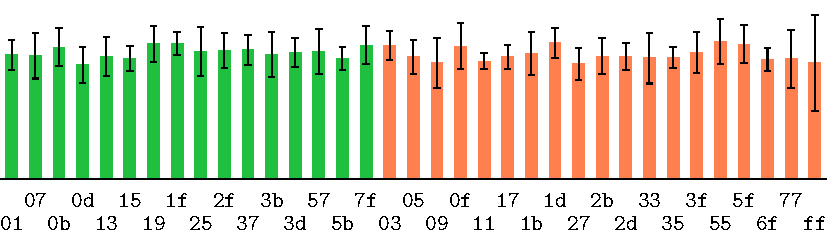
\includegraphics{figures/leak_target/leak_target.pdf}
		\caption{Success rate by targets' corresponding $p$'s and their standard deviation. Green represents invertible $p$'s, orange noninvertible ones.}
		\label{fig:leaktargethist}
	\end{center}
	\end{figure}
	
	%~ Note high deviation at {\tt ff}, this is because there is only a single target in this group (one generated by $B^T = (1,1,1,1,1,1,1,1)$).   %!% totál blbost, dev se přece nemůže zlepšovat počtem měření ne?
	Note that we did not give $y$-axis scale since the purpose is only to distinguish uniform distribution.
	
	\paragraph{Group with fixed $4$ bits in $B$.}
	
	Another way of grouping we performed, groups targets by fixing $4$ out of $8$ bits of their corresponding vector $B$, see Equation \ref{eq:tba}. We fixed the first and the last $4$ bits and grouped them, see results in Figure \ref{fig:leaktargetotherhist}, where these ways of grouping are in green or orange, respectively. Group index can be computed as binary AND of mask {\tt 0xf0} or {\tt 0x0f} with vector $B$, respectively.
	
	\begin{figure}[h]
	\begin{center}
		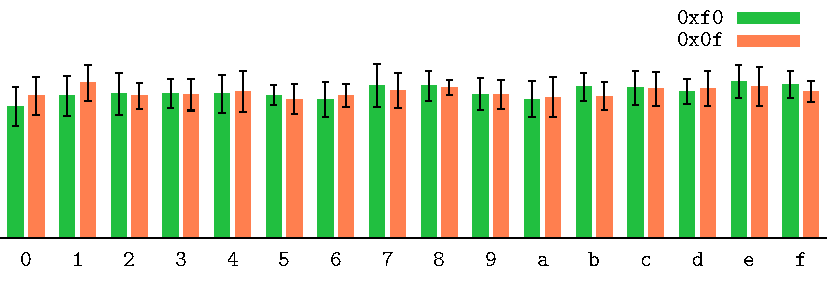
\includegraphics{figures/leak_target_other/leak_0x0f_0xf0.pdf}
		\caption{Success rate by fixed $4$ bits of targets' corresponding vector $B$. Green represents fixed first $4$ bits, orange represents last $4$ bits.}
		\label{fig:leaktargetotherhist}
	\end{center}
	\end{figure}
	
	\begin{remark}
	\label{rem:uniform}
		According to our observations, there does not seem to be a preferred target or a group of targets, therefore we will assume that target success rate is constant across all targets.
	\end{remark}

\subsubsection{False Positives}
	
	There is an inconvenience which emerges once we do not know the key -- we do not recognize the correct candidate anymore (see Remark \ref{rem:false}). Therefore we observed behavior of the incorrect ones.
	
	\paragraph{Gaps of incorrect candidates.}
		
		Previously we defined a strong candidate as a candidate with a gap larger than $10\%$. Most candidates which exceeded this limit were also correct candidates, but there were a couple of exceptions which we will refer to as {\em false positives}. Note that $25\%$ of candidates were strong and correct, on the other hand, there were $11\%$ of strong and incorrect ones. On average, strong incorrect candidates had a gap of $14\%$ (cf.\ $40\%$ for correct ones) and the highest gap ever seen was $35\%$ (cf.\ $76\%$ for correct ones). We need another observation about incorrect candidates in order to distinguish them from the correct ones.
		% 1024:
		% strong & correct:
		% 	[1019, 1000, 978, 1008, 986, 1006, 1019, 999] => 1001.875 ... 24.6%
		% 	[39.46, 39.68, 39.5, 40.28, 40.2, 39.85, 39.86, 39.68] => 39.81375
		% strong & incorrect:
		% 	[442, 440, 425, 415, 433, 463, 413, 468] => 437.375 ... 10.7%
		% 	[14.05, 14.06, 14.16, 13.95, 14.26, 13.83, 14.0, 13.97] => 14.035
	
	\paragraph{Number of repetitions of strong incorrect candidates.}
		
		The good news is that incorrect candidates do not repeat among targets very often. We observed the number of most repeating strong incorrect candidates among our $255$ targets and got following results: on average, the number was $1.75$, the maximum was $3$.
		% 	[1.88, 1.75, 1.81, 1.81, 1.62, 1.88, 1.62, 1.62]

\subsubsection{Using Less Traces}
	
	So far we used $1024$ traces in our attack, let us have a look at results of the attack with much less traces. Note that Bos et al.\ \cite{bos2015differential} used $2000$ and $500$ traces for the attack targetting the original SBox and Rijndael inverse, respectively.
	
	We used also much less traces, namely $128$, $256$, $384$ and $512$. For each number of traces we attacked all of our $8$ instances of {\tt KlinecWBAES} and observed success rate of strong candidates and their average gap. See results in Table \ref{tab:ntraces}.
	
	\begin{table}[h]
		\begin{center}
		\begin{tabular}{| c | c | c | c | c | c | c | c |}
			\hline
			Traces       &    $128$ &    $256$ &    $384$ &   $512$ &   $1024$ \\
			\hline
			Success rate &  $9.8\%$ &   $17\%$ &  ?       & ?       &   $25\%$ \\
			\hline
			Average gap  &   $24\%$ &   $32\%$ &  ?       & ?       &   $40\%$ \\
			\hline
			Reduced cost\footnote{Will be introduced later.}
			             & $5\,400$ & $4\,700$ & $.$ & $.$ & $10\,500$ \\
			\hline
		\end{tabular}
		\end{center}
	\caption{Success rates and average gaps using different numbers of traces.}
	\label{tab:ntraces}
	\end{table}
	
	% 128:
	% strong & correct:
	% 	[388, 420, 391, 411, 402, 393, 412, 397] => 401.750 ... 9.8%
	% 	[24.23, 24.39, 24.26, 23.65, 24.5, 24.01, 23.87, 23.65] => 24.07
	% strong & incorrect:
	% 	[262, 325, 351, 322, 309, 342, 285, 315] => 313.875 ... 7.7%
	% 	[13.34, 13.34, 13.13, 13.12, 12.9, 13.22, 13.26, 13.33] => 13.205
	
	% 256:
	% strong & correct:
	% 	[700, 670, 658, 722, 700, 709, 707, 683] => 693.625 ... 17.0%
	% 	[31.74, 32.49, 32.41, 31.83, 32.29, 31.31, 31.91, 32.11] => 32.01125
	% strong & incorrect:
	% 	[431, 472, 423, 441, 447, 451, 424, 482] => 446.375 ... 10.9%
	% 	[13.82, 13.85, 13.69, 14.1, 14.01, 14.1, 13.95, 14.36] => 13.985
	
	% 384:
	% strong & correct:
	% 	[814,791,784,825,790,819,812,]
	% 	[35.84,35.59,35.14,35.26,36.19,35.26,35.77,]
	% strong & incorrect:
	% 	[491,488,484,504,487,464,509,]
	% 	[14.17,14.37,13.97,14.17,14.14,14.07,14.23,]
	
	% 512:
	% strong & correct:
	% 	[879,851,855,887,848,]
	% 	[37.25,37.47,36.58,37.66,38.04,]
	% strong & incorrect:
	% 	[471,480,473,478,472,]
	% 	[14.02,14.09,13.96,13.97,14.23,]

\subsubsection{Leaking Bits}
	
	Remind that our trace is a bit-wise serialization of least significant bytes of memory addresses, hence we can identify which bit within that byte leaked -- simply by taking the leaking position within trace modulo $8$. This moduled position will be referred to as {\em leaking bit} (note the difference from target bit).
	
	We noticed soon that leaking bits are not very well balanced (as one would expect), therefore we put this data into a histogram, see Figure \ref{fig:leakbitall}. The histogram shows the amount of correct candidates with a gap larger than $10\%$ averaged over $8$ WBAES instances, for each leaking bit, together with standard deviation which is surprisingly very low. Note that the histogram does not provide absolute values since these could be misleading, only distribution is relevant at the moment.
	
	\begin{figure}[h]
	\begin{center}
		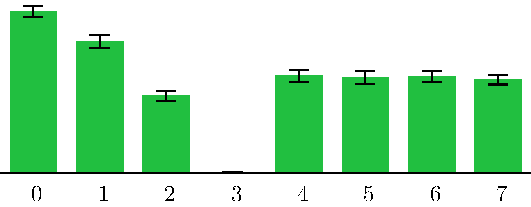
\includegraphics{figures/leak_bit/leak_bit.pdf}
		\caption{Average number of leaks and its standard deviation at each bit within trace.}
		\label{fig:leakbitall}
	\end{center}
	\end{figure}
	
	The \nth{0} and \nth{1} bits leaked slightly more, the \nth{2} bit slightly less and the \nth{3} bit actually leaked only twice while the overal average of the remaining bits was almost $160$! On the other hand, all of the remaining bits leaked fairly similarly. We do not have any explanation for this behavior.


% ==============================================================================
% ===   B L I N D   A T T A C K   S U G G E S T I O N                        ===
% ==============================================================================

\subsection{Blind Attack Suggestion}
\label{sec:subblindattack}

\begin{note}
	This section only applies previous observations on a heuristic basis, there is no guarantee that our approach is the best.
\end{note}

In general, we suggest to use rather less traces and repeat the attack with several targets until the sum of strong gaps of any candidate exceeds given bound.

According to results in Table \ref{tab:ntraces}, we attempt to estimate convenient number of traces. For this reason, we introduce {\em reduced cost of gap}, defined as
\begin{equation}
\label{eq:redcost}
	C(n, s, g) = \frac{n}{s\cdot g} ,
\end{equation}
where $n$ stands for the number of traces, $s$ for average success rate and $g$ for average gap of a strong candidate. Note that this quantity corresponds with average time of the attack: the more traces, the longer time; the better success rate or the bigger gap, the shorter time. Thus we can use this measure to compare expected time of the attack using different number of traces.


% omitting strong candidates' bound leads to ~1.5\% enhancement

% We rather suggest the following:
%~ \begin{enumerate}
	%~ \item pick a target, %?% Chi-square test of uniformity, pick random
	%~ \item attack using $256$ traces
%~ \end{enumerate}
% 10\% pro započtení, 75\% kumulativní mez? moc často se totiž neopakujou
% vyzkoušet jestli tak zlomim všechny instance

%~ Therefore, in case of blind attack (i.e.\ no knowledge of actual key), we suggest to use less traces, but keep changing the target until the maximal gap exceeds $27\%$, then we accept that candidate. This is likely to happen soon since $10.6$ out of $16$ targets succeed on average.

% psal já / Teuwen:
%~ > I only wonder about the reasoning why Karroumi is more than Chow since
%~ > it seems to have been shown to be equal (based on what I wrote in my
%~ > previous email).
%~ 
%~ Well I've no problem to break completely Chow with standard DCA so there
%~ is something a bit more in Karroumi. Obviously not enough to make it
%~ robust enough...


\section{Use in White-Box Cryptography Design}
\label{sec:useindesign}

The benefit of this attack is obvious -- it introduces a principially different approach to break white-box cryptography implementations. This attack may help to address weaknesses of any future white-box cryptography implementation and possibly increase its resistance to this kind of attack.

So far, we were only interested in results of the attack. In this section, we will study practical consequences of the attack itself. First we describe our initial effort trying to identify which intermediate product causes the leakage, then we outline some countermeasures against this attack. Both might be useful in white-box cryptography design.


% ==============================================================================
% ===   P O I N T   O F   L E A K A G E                                      ===
% ==============================================================================

\subsection{Point of Leakage}
\label{sec:leakpoint}

Note that the attack allows us to reveal concrete addresses which contributed to the key recovery. Our original intention was to find the corresponding piece of source code, and possibly deduce the intermediate product, which is later transformed into leaking memory address, -- it would most likely be used as an array index.

We tried two ways of using a debugger how to find that position in source code, but neither of them gave any results. Authors of the DCA toolkit \cite{bos2016tools} were successful at this point, see their comprehensive and very technical report on a wiki page of their Deadpool repository\footnote{Direct link:\\\link{github.com/SideChannelMarvels/Deadpool/wiki/Tutorial-\%234\%3A-DCA-against-Karroumi-2010-challenge}.\\Accessed 2016-04-24.}.

One could possibly try yet another approach -- modify the source code to output directly all relevant array indexes. Note that it might be challenging to address them really all.

However, we did not finally make use of this information (i.e., the point of leakage in source code) -- we identified the leaking intermediate product rather by a mathematical reasoning. This will be given in Section~\ref{sec:attempt}.

% LEGACY !!!
% BEGIN
%~ \begin{description}
	%~ \item[Watchpoint in GDB.]
		%~ We acquired one full trace (as described in Section~\ref{sec:filter} under the caption ``\nameref{subsec:atf}'') for some plaintext used during the acquisition phase. We checked that this trace perfectly matches the corresponding trace from the acquisition phase.
		%~ 
		%~ We identified the leaking address and set up a watchpoint in GDB running in the same terminal session. However, GDB did not catch the address, probably because PIN uses different virtual environment.
	%~ \item[GDB connected to PIN's debugging interface.]
		%~ We set up a connection between PIN application debugging interface and GDB as described in PIN manual \cite{pin214manual}, but could not catch {\em any} address. GDB was complaining that it cannot insert hardware breakpoint, on the other hand, software breakpoints did not work either.
	%~ \item[Outputting all array indexes.]
		%~ Note that array indexes are very likely the values which are later transformed into leaking memory addresses. Hence it should be possible to output and attack all indexes used within the encryption procedure. However we did not succeed with the first attempt -- it required certain reasoning and finding the specific intermediate result to output; both will be given in Section~\ref{sec:attempt}.
%~ \end{description}
% END


% ==============================================================================
% ===   C O U N T E R M E A S U R E S   A G A I N S T   D C A                ===
% ==============================================================================

\subsection{Countermeasures against DCA}

Since DCA is based on an algorithm, which was originally developed for physical measurements of certain hardware emissions, we can look for some inspiration back in hardware model. There are several countermeasures, see the following list for some of them (basic ones are introduced in \cite{chari1999towards,goubin1999des}).
\begin{description}
	\item[Masking with random values.] Cryptographic hardware can run some unpretendable source of random data and thus mess up values in traces (i.e., adding a strong noise). However, there is no equivalent of noise in white-box context, since everything is is fully controlled by the attacker.
	\item[Reordering instructions.] Remind that our algorithms required aligned traces, therefore it would be fatal if the leaking position were at several different places. However, this could be possibly overcome in white-box context -- we could achieve this by reverse engineering or, much easier, by aligning the traces with respect to instruction address trace (as outlined by Bos et al.).
	\item[Adding random delays.] Note that random delays have very similar properties as the previous countermeasures -- it can be controlled by the attacker and it only causes a trace misalignment.
\end{description}
In general, we cannot rely on any source of {\em dynamic} random data (generated during program execution). All we need to rely on is {\em static} random data (generated during instantiation). On the other hand, dynamic randomness can be used in a white-box implementation -- just as another level of ``obfuscation''.

Bos et al.\ further propose to use some ideas from {\em threshold implementations} \cite{nikova2006threshold} or use of external encodings -- here they emphasize that more research is needed.


\section{Explanation Attempt}
\label{sec:attempt}

First of all, let us remind the information flow through WBAES tables (originally in Equation \ref{eq:wbaesflow}), especially its first table.
\begin{equation}
\label{eq:wbaesfirst}
	\ldots \rarr \underbracket{\Enc \rarr \IMB^{-1} \xrightarrow{\textnormal{plain}} \TBox \xrightarrow{\textnormal{plain}} \MB \circ \MC \rarr \Enc^{-1}}_{\textnormal{in table}} \rarr \ldots
\end{equation}
Note that the last plain AES state (denoted with ``plain'' in the previous equation) is actually an $8$-bit output of the first SBox i.e.\ the very original target. Let us see what happens next: a composed linear mapping $\MB\circ\MC$ is applied resulting in a $32$-bit output (using an idea outlined in Section \ref{sec:aeslookup}), then each $4$-bit nibble is passed through a $4$-bit random bijection $\Enc^{-1}$ (further simply $\Enc$).

\begin{description}
	\item[$\MB\circ\MC$.] We can view each bit $t$ of the $32$-bit output of $\MB\circ\MC$ as a scalar product of a row $[R]^T$ of matrix representing $\MB\circ\MC$ (i.e.\ a random-like\footnote{Cannot be zero (follows from Note \ref{note:fullrank}).} $8$-bit vector) with its $8$-bit input $[S]$ which is actually an output of the first SBox. We get
	\begin{equation}
		t = [R]^T\cdot [S] = [R]^T\cdot\Bigl( \{\texttt{1f}\}\cdot\bigl([K]+[P]\bigr)' + [\texttt{63}] \Bigr) ,
	\end{equation}
	where $\{\cdot\}$ stands for respective binary matrix of multiplication modulo $x^8+1$ and $(\cdot)'$ for Rijndael inverse (i.e.\ there is the output of the first SBox in the big parantheses, cf.\ Equation \ref{eq:sbox}). This equation can be easily turned into the form of previously used target (Equation \ref{eq:tba}), indeed
	\begin{align*}
		[R]^T\cdot\Bigl( \{\texttt{1f}\}\cdot\bigl([K]+[P]\bigr)' + [\texttt{63}] \Bigr) &= \bigl([R]^T\cdot \{\texttt{1f}\}\bigr)\cdot\bigl([K]+[P]\bigr)' + \bigl([R]^T\cdot [\texttt{63}]\bigr) = \\
		&= [\bar R]^T \cdot \bigl([K]+[P]\bigr)' + \bar r ,
	\end{align*}
	where $\bar R$ is just a different random-like vector, which plays the role of $B$ in Equation \ref{eq:tba}, and $\bar r$ is a constant bit. Remind that additive constant does not need to be considered inside target (see Remark \ref{rem:pqeffect}). It follows that each of these $32$ bits perfectly matches some of our $255$ targets introduced in Section \ref{sec:unify}.
	
	%!% nebylo tu, zakamuflovat
	Note that, even though $\MB\circ\MC$ introduces diffusion, there is no diffusion so far, because those $32$-bit intermediate results are not combined together so far. Therefore these intermediate results only depend on single input byte!
	
	If we could observe these intermediate results, we would get the difference of means equal to $1.0$ (cf.\ attack against unprotected implementation in Section \ref{sec:naiveaes}).
\end{description}
\begin{remark}
\label{rem:enc}
	It follows that the protection against our $255$ targets is fully and solely accomplished by $\Enc$.
\end{remark}
\begin{description}
	\item[$\Enc$.] Remind that $\Enc$ is a (only) $4$-bit random bijection. Note that, unlike confusion elements in regular ciphers (e.g.\ SBox in AES), there is no nonlinearity check\footnote{Linearity in ciphers is studied by {\em linear cryptanalysis}, see e.g.\ \cite{matsui1993linear} for detail.} in WBAES by Chow et al.\ \cite{chow2002aes}.
	
	The choice of $\Enc$ actually only relies on the fact that the ratio of affine mappings among all random bijections is extremely low (less than $0.000\,002\%$ for $4$-bit bijections). This justification is very poor since it does not even address the case where only one output bit of $\Enc$ is an affine mapping of the input!
	
	There are actually quite many bijections which are affine in single output bit. Indeed, there are $2\cdot4\cdot(2^4-1)\cdot8!\cdot8! \approx 2\cdot10^{11}$ of them among $16! \approx 2\cdot10^{13}$ bijections on $4$-bits altogether which already makes some $1\%$ ratio! Also note that in such case, the maximum difference of means would be still $1.0$ since this affine mapping could be composed with the previous affine mappings yielding an affine mapping again.
	
	But we do not necessarily need a fully affine mapping at some bit, it would be sufficient if the mapping were affine for most inputs. Clearly, there are much more such mappings. For this reason, this intermediate result of WBAES seems to be most likely that which causes the leakage.
\end{description}

To support our hypothesis, we modified the source code of {\tt KlinecWBAES} to output these intermediate products (i.e.\ outputs of the first Type II tables, see Equation \ref{eq:wbaesflow}) and ran the attack with these values instead of memory traces. The attack indeed succeeded, which fully supports our explanation.

However, we noticed an interesting thing: leaking bits, as introduced in Note \ref{note:leakbit}, appear to be uniform in this case!

% perla (jakože fakt nebrat vážně): Note that a random bijection is extremely unlikely to provide any correlation between any input and output bit.


   % kéž by ...
		
		%%% KAPITOLA 5
		\chapter{Future Work}
\label{chap:future}

\section{Another Interesting AES White-Box Implementation}
\label{sec:magicimpl}

Bos et al.\ \cite{bos2015differential} mention another interesting AES white-box implementation in their paper. This particular implementation by Eloi Vanderbéken was first published only as a Windows binary executable challenge at NoSuchCon 2013 conference\footnote{\link{http://www.nosuchcon.org/2013/}}, where nobody was able to recover the key. Note that this implementation uses an externally-encoded variant of AES (as outlined in Section \ref{sec:constrwbaes}, in particular in Equation \ref{eq:extenc}), hence it is {\em not compliant with AES anymore}. It follows that any SCA-like attack is impossible, since the internal AES handles encoded inputs, where the encoding is unknown.

Soon after the conference, the author released source codes\footnote{\link{http://pastebin.com/MvXpGZts}}, which allows one to avoid reverse engineering of the binary. Moreover, it allows one to modify the code to run natively on Linux. Philippe Teuwen, a co-author of Bos et al.\ \cite{bos2015differential}, studied this implementation deeper and finally was able to recover the key \cite{teuwen2015nscwriteups}.

In his write-up, Teuwen also describes the structure, which appears to avoid usage of $4$-bit random bijections (in WBAES by Chow et al.\ \cite{chow2002aes}) and uses $8$-bit ones instead. Note that even without any non-linearity check, it is far less likely that any bit of output of a random $8$-bit bijection would provide a reasonable level of linearity compared to a random $4$-bit bijection, as outlined in Section \ref{sec:attempt}.

However, we did not either modify the source code to make it AES-compliant, nor did run the attack, hence it remains as a possible topic for further research.

%?%
% \section{What next?}
		
		%%% ZÁVĚR
		% cleardoublepage and phantomsection force that link jumps ABOVE heading, normally it would jump UNDER heading
\cleardoublepage\phantomsection

\addcontentsline{toc}{chapter}{Conclusion}
\chapter*{Conclusion}
\markboth{\MakeUppercase{Conclusion}}{}

%!% finish this chapter ...
%~ After an introduction to white-box cryptography, side-channel attack scenario and \ldots in Chapter~\ref{chap:intro} we blah blah.
%~ 
%~ Another interesting problem which arised during \ldots is described within Section blah. This problem might be a direction of future research.

% reproduced, enhanced and gave a simplifying framework
% identified & confirmed leaking intermediate product solely by analysis of WBAES
% hence identified the weakest link of WBAES (remark ...)
% avoids reverse engineering \ref{rem:benefit}
		
		%%% LITERATURA
		% cleardoublepage and phantomsection force that link jumps ABOVE heading, normally it would jump UNDER heading
\cleardoublepage\phantomsection

\addcontentsline{toc}{chapter}{\bibname}

\bibliographystyle{plain}
\bibliography{biblio}

		
		%%% APPENDIX
		\setcounter{tocdepth}{0}
\begin{appendices}

\chapter{Contents of Attached CD}
\pagenumbering{Roman}
\label{app:cd}
	
	\begin{description}
		\item[\tt README] ~ \\ README file,
		\item[\tt diploma-thesis.pdf] ~ \\ diploma thesis in Portable Document Format,
		\item[\tt implementations/] ~ \\ folder with (white-box) AES implementations,
		\item[\tt implementations/naiveAES/] ~ \\ Git repository -- sources of our naive AES implementation,
		\item[\tt implementations/klinecWBAES/] ~ \\ Git repository -- sources of Klinec's WBAES implementation \cite{klinec2013implementation},
		\item[\tt implementations/???/] ~ \\ source of magic AES white-box implementation introduced in Section~\ref{sec:magicimpl},
		\item[\tt attack/] ~ \\ Git repository -- our attack scripts written in Ruby,
		\item[\tt cpp\_attack/] ~ \\ Git repository -- sources of our side-channel attack tool implementing a primitive of Algorithm~\ref{alg:bitwisedpa} and its further modifications,
		\item[\tt data/] ~ \\ folder with comprimed traces and respective results of our $8$ instantiations,
		\item[\tt .] ~ \\ \ldots
	\end{description}


%~ \chapter{User Guide}
\label{app:guide}

%!% finish it!
%~ \section{Get a White-Box AES Binary}
%~ \label{sec:getbinary}
	%~ 
	%~ Download or git-clone your desired white-box implementation, e.g.\ Klinec's one. If needed, modify it so that it only performs encryption with an embedded key.
%~ 
%~ \section{Install a Memory-Tracing Tool}
%~ \label{sec:install-tool}
	%~ 
	%~ Install Pin, copy the memory tracing tool from our CD or github, make the tool.
%~ 
%~ \section{Acquire Memory Traces}
%~ \label{sec:acquire}
	%~ 
	%~ Use our script.
%~ 
%~ \section{Run Attack}
%~ \label{sec:run-attack}
	%~ 
	%~ Run attack and find the address where it leaks. Note that the address depends on input.
%~ 
%~ \section{Find Leakage}
	%~ 
	%~ (Optional -- only if source code is available) Run in GDB, set a memory-breakpoint on that address and find the line of code where it leaks. You can use this information for future analysis.   %?%

\end{appendices}
		
		
%%%%%%%%%%%%%%%%%%%%%%%%%%%%%%%%%%%%%%%%%%%%%%%%%%%%%%%%%%%%%%%%%%%%%%%%
%%%   K O N E C   P R Á C E
%%%%%%%%%%%%%%%%%%%%%%%%%%%%%%%%%%%%%%%%%%%%%%%%%%%%%%%%%%%%%%%%%%%%%%%%


\end{document}